%Preambolo per documento generico
%Per cambiare tipo di documento modificare
%il documentclass.

\documentclass[11pt]{article}
\usepackage[utf8]{inputenc}

%Mettere italian se si vuole scrivere in italiano
\usepackage[english]{babel}


%Aumento dell'interlinea
\usepackage{setspace}
\onehalfspacing

%Pacchetti per simboli matematici
\usepackage{mathtools}
\usepackage{amsfonts}
\usepackage{amsthm}
\newtheorem{theorem}{Theorem}
\usepackage{amsmath}
\usepackage{bm}
\usepackage{mathrsfs}



%Pacchetti per figure e tabelle
\usepackage{booktabs, caption, graphicx, subfig, float}
\captionsetup{tableposition=top,figureposition=bottom,font=small}

%Per inserire commenti in blocco
%Usage: \begin{comment} ... \end{comment}
\usepackage{comment}

%Definisce colori dei link nel testo e altri parametri
\usepackage{hyperref}
\hypersetup{
pdftitle={AMR Project - Hybrid Zero Dynamics},%
pdfauthor={De Filippis, Tantucci, Wrona},%
pdfsubject={},%
pdfkeywords={},%
colorlinks=true,%
linkcolor=black,%
linktocpage=true,%
pageanchor=true,
citecolor=black
}

%Definisce in maniera simmetrica i margini di pagina
\usepackage{geometry}
\geometry{a4paper, top=3cm,bottom=2cm,left=3cm,right=3cm,%
			heightrounded}

%Per scrivere in maniera rapida norme e valori assoluti
%Usage: y = \abs{x} ; y = \norma{x}
\DeclarePairedDelimiter{\abs}{\lvert}{\rvert}
\DeclarePairedDelimiter{\norma}{\lVert}{\rVert}

%Testo a caso
%Usage: \lipsum[a-b]
%\usepackage{lipsum}

%Cambia lo stile della pagina
%In alto a dx mette numero di pagina
%In alto a sinistra titolo e autore
\usepackage{fancyhdr}
\pagestyle{fancy}
\fancyhf{}
\rhead{\textit{\thepage}}
\lhead{\textit{}}

%Per inserire codice nativo MATLAB e simili
%Usage: guardare sotto
\usepackage{fancyvrb}


\begin{document}

\title{Autonomous and Mobile Robotics Report - Project \#3\\}
\author{Stefano De Filippis, Andrea Tantucci, Andrea Wrona}
%Optional: data. Se non si inserisce il campo data
%LaTeX mette la data del PC automaticamente

\maketitle

\thispagestyle{empty}

%Inizio dei capitoli
\section*{Introduction}

A planar biped walker is a robot which locomotes via alternation of the contact points of the two legs with the ground in the sagittal plane (see \figurename\, \ref{fig: planar biped walker}). The models for this kind of robot are necessarily hybrid, consisting of ordinary second order differential equations which describe the motion of the robot when only one leg is in contact with the ground (single support phase), and a discrete map to model the passage from a single support phase to another one.

\begin{figure}[H]
\centering
\includegraphics[width=.6\textwidth]{Images/Planar_biped_walker.png}
\caption{Representation of a high DOF biped walker. Cartesian coordinates are indicated at the hips and the leg ends}
\label{fig: planar biped walker}
\end{figure}

The aim of this work is to study the gait generation via hybrid trajectory optimization and feedback linearization, and to compare the results with another kind of gait generation, based on Center of Mass (CoM) trajectory and differential kinematics tracking. 

The report is organized as follows. In Sec. 1 the robot model and the modeling assumptions are presented. In Sec. 2 the case study is described in detail, that is the RABBIT robot. In Sec. 3 a hybrid trajectory optimization approach which makes use of the FROST toolkit is presented. In Sec. 4 an algorithm to generate CoM trajectories and the tracking via differential kinematics is reported. Eventually, in Sec. 5 the results of the two approaches on the case study are shown\part{reported} and a comparison between them is developed.

\section{Robot Model and Model Assumptions}

The model considered is an open kinematic chain connected at a single joint called \textit{hip}, comprising two identical open kinematic chains called \textit{legs} and a third one called \textit{torso}. It is assumed that the transition from one leg to the other takes an infinitesimal amount of time. This entails the use of a rigid contact model to describe the impact of the swing leg to the ground which presents a discontinuity in the velocity component of the state. It follows that the model is indeed hybrid, consisting of a continuous dynamics and a re--initialization rule at the contact event.

Before describing the equations which characterize a biped walker, a series of hypotheses on the model itself and on the desired walking gaits are presented.

\textit{\textbf{Robot Hypothesis}}: The robot is supposed to be:
\begin{description}
\item[RH1] comprised of \textit{N} rigid links with mass, connected by revolute joints with no closed kinematic chains;
\item[RH2] planar, with motion constrained to the sagittal plane;
\item[RH3] bipedal, with identical legs connected at a common point called the hips;
\item[RH4] actuated at each joint;
\item[RH5] unactuated at the point of contact between the stance leg and ground.
\end{description}

\textit{\textbf{Gait Hypothesis}}:

\begin{description}
\item[GH1] There are alternating phases of single support and double support;
\item[GH2] During the single support phase, the stance leg acts as a pivot joint, that is, throughout the contact, it can be guaranteed that the vertical component of the ground reaction force is positive and that the ratio of the horizontal component to the vertical component does not exceed the coefficient of static friction;
\item[GH3] The double support phase is instantaneous and can be modeled as a rigid contact;
\item[GH4] At impact, the swing leg neither slips nor rebounds;
\item[GH5] In steady state, successive phases of single support are symmetric with respect to the two legs;
\item[GH6] Walking is from left to right, so that the swing leg starts from behind the stance leg and is placed strictly in front of the stance leg at impact.
\end{description}

It is possible to identify two different models for the biped walker: the \textit{Swing Phase Model}, which characterizes the swing phase of the robot and the \textit{Impact Model} which describes the double contact phase and is characterized by both dynamical equations and the relabeling phase.

\subsection{Swing Phase Model}

Let $q \coloneqq [q_1,\, q_2, \ldots \, ,q_N]'$ be a set of angular coordinates describing the configuration of the robot. Using the Lagrangian approach, for one leg, one gets 
\begin{equation}
D(q)\ddot{q} + C(q,\dot{q})\dot{q} + G(q) = Bu
\end{equation}
where $D(q)$ is the inertia matrix, $C(q,\dot{q})$ is the term which collects the Coriolis and centrifugal terms, $G(q)$ is the gravity vector, $B$ is the input matrix and $u$ is the torque input. Since only symmetric gaits are of interest, this model can be used for both legs with a proper relabeling after the contact phase.

The control input has $N-1$ components by hypothesis: the input is not applied between the stance leg and the ground. The model can be written in state--space form
\begin{equation}
\dot{x} = 
\begin{bmatrix}
\dot{q}\\
D^{-1}(q)[-C(q,\dot{q})\dot{q} -G(q) +Bu]\\
\end{bmatrix}
\end{equation}
which is a nonlinear system of the form
\begin{equation}
\dot{x} = f(x) + g(x)u
\end{equation}
where $x \coloneqq [q, \, \dot{q}]'$. The state space of the model is taken as $TQ \coloneqq \{x \coloneqq [q,\dot{q}]\vert q \in \mathcal{Q}, \dot{q} \in \mathbb{R}^N\}$, where $\mathcal{Q}$ is a simply connected, open subset of $[0, 2 \pi]^N$ corresponding to physically reasonable configurations of the robot.

\subsection{Impact Model}

The impact between the swing leg and the ground is assumed to be an interaction between rigid bodies and the model needs to take into account the relabeling of the coordinates when one builds the equations. In particular, the coordinates before the impact are indicated with the superscript ``$-$'', whereas the ones after the relabeling are indicated with the superscript ``$+$''.\\
The definition of this model requires the full $(N+2)$--DOF of the robot, so by augmenting the configuration with the coordinates of the hip $[p^h_H\,p^v_H]$, which are the ones represented in \figurename \,\ref{fig: planar biped walker}, the model which is obtained is the following
\begin{equation}
D_e(q_e)\ddot{q}_e + C_e(q_e,\dot{q}_e)\dot{q}_e + G_e(q_e) = B_eu + \delta F_{ext}
\label{extModel}
\end{equation}
where $q_e \coloneqq [q',p^h_H,p^v_H]'$ and $\delta F_{ext}$ represents the vector of external forces acting on the robot at the contact point. The extended coordinates $q_e$ and $\dot{q}_e$ are related to the previous ones $q$ and $\dot{q}$ by the following relations
\begin{align*}
q_e &= \Upsilon(q) & \dot{q}_e &= \dfrac{\partial \Upsilon}{\partial q}\dot{q}
\end{align*}
where $\Upsilon(q) \coloneqq [q',p^h_H(q),p^v_H(q)]'$. There are some assumptions which need to be done in order to use this model.

\textit{\textbf{Impact Model Hypothesis}}:
\begin{description}
\item[IH1] The contact of the swing leg with the ground results in no rebound and no slipping of the swing leg;
\item[IH2] At the moment of impact, the stance leg lifts from the ground without interaction;
\item[IH3] The impact is instantaneous;
\item[IH4] The external forces during the impact can be represented by impulses;
\item[IH5] The impulsive forces may result in an instantaneous change in the velocities, but there is no instantaneous change in the configuration;
\item[IH6] The actuators cannot generate impulses and so they can be ignored during impact.
\end{description}

It can also be defined a relation between the velocities of the coordinates before and after the impact (without relabeling) which is the following:
\begin{equation}
\Pi^{-1} (q^-_e)
\begin{bmatrix}
\dot{q}^+_e \\
F^T_2 \\
F^N_2 \\
\end{bmatrix}
= 
\begin{bmatrix}
D_e(q^-_e)\dot{q}^-_e \\
0
\end{bmatrix}
\end{equation}
where 
\begin{equation*}
\Pi(q_e) \coloneqq
\begin{bmatrix}
D_e(q_e) & - \Bigl(\dfrac{\partial E(q_e)}{\partial q_e} \Bigr)' \\
\dfrac{\partial E(q_e)}{\partial q_e} & 0 \\
\end{bmatrix}^{-1}
\end{equation*}
where $E(q_e) = [p^h_2(q_e),p^v_2(q_e)]'$ are the cartesian coordinates of the end of the swing leg and $F^T_2$, $F^N_2$ are respectively the integrals of the tangential and normal contact impulsive forces.
Since the inverse of the matrix exists, then the previous relation becomes
\begin{equation}
\begin{bmatrix}
\dot{q}^+_e \\
F^T_2 \\
F^N_2 \\
\end{bmatrix}
= 
\Pi(q^-_e)
\begin{bmatrix}
D_e(q^-_e)\dot{q}^-_e \\
0
\end{bmatrix}
\end{equation}
From this the mapping of the velocities can be extracted
\begin{equation}
\dot{q}^+_e = \Pi_{11}(q^-_e)D_e(q^-_e)\dot{q}^-_e
\end{equation}

The relabeling of the coordinates can be expressed by a linear invertible transformation matrix $R$ and the final expression is
\begin{equation}
x^+ = \Delta(x^-)
\end{equation}
where $x^+ \coloneqq [q^+,\dot{q}^+]$, (respectively $x^- \coloneqq [q^-, \dot{q}^-]$) and 
\begin{equation}
\Delta(x^-) =
\begin{bmatrix}
\Delta_q q^- \\
\Delta_{\dot{q}}(q^-) \dot{q}^-
\end{bmatrix}
\end{equation}
where $\Delta_q \coloneqq R$ and $\Delta_{\dot{q}}(q^-) \coloneqq \bigl[
\begin{matrix}
R & 0
\end{matrix}\bigr]$
$\Pi_{11}(\Upsilon(q^-))D_e(\Upsilon(q^-))\dfrac{\partial \Upsilon(q)}{\partial q}\vert_{q = q^-}$.

\subsection{Plant Model}
Based on the previous discussions, the overall model of the biped robot can be expressed as a nonlinear sysem with impulse effects
\begin{align}
\dot{x} &= f(x) + g(x)u, & x \notin S \\
x^+ &= \Delta(x^-), & x \in S 
\end{align}
where 
\begin{equation*}
S \coloneqq \{(q,\dot{q}) \in TQ\vert p^v_2(q) = 0, p^h_2(q) >0\}
\end{equation*}
The reason why $p^h_2(q)$ is taken greater than zero is to respect the hypothesis for which, at impact, the swing leg is right in front of the stance leg (GH6).

\section{Case Study}
The robot which is taken into account is the prototype RABBIT (see \figurename \, \ref{fig: RABBIT_color}), which is a five-link robot built during the French project \textit{Commande de Robotsà Pattes of the CNRS—GdR Automatique}. 

\begin{figure}[H]
\centering
\includegraphics[width=.32\textwidth]{Images/RABBIT_color.png}
\caption{RABBIT prototype}
\label{fig: RABBIT_color}
\end{figure}

The configuration variables are five $q \coloneqq [q_1, q_{31}, q_{32}, q_{41}, q_{42}]$, where $q_1$ represents the torso displacement with respect to the vertical axis, $q_{31}$ and $q_{32}$ represent respectiveley the stance leg and the swing leg femur displacements with respect to $q_{1}$, $q_{41}$ and $q_{42}$ represent respectively the stance leg and the swing leg tibia displacements with respect to the femurs longitudinal axes. This configuration is shown in \figurename \, \ref{fig: RABBIT}. 

\begin{figure}[H]
\centering
\includegraphics[width=.45\textwidth]{Images/RABBIT.png}
\caption{RABBIT configuration variables representation}
\label{fig: RABBIT}
\end{figure}

The robot is underactuated and equipped with four electric DC motors which allow simpler control, higher bandwidth and easier construction than pneumatic or hydraulic drives. Moreover, a gearbox is used to connect the motors with the four actuated joints. Here is also presented the table of kinematic and dynamic parameters for RABBIT.\\
\begin{table}[H]
\centering
\caption{Table of RABBIT parameters}
\begin{tabular}{cccc}
\toprule
Model  & Torso & Femurs & Tibias \\
Parameters & (T) & (\textit{f}) & (\textit{t})\\
\midrule
Mass, $M_*$ ($kg$) & $20$ & $6.8$ & $3.2$ \\
Lenght, $L_*$ ($m$) & $0.625$ & $0.4$ & $0.4$\\
Inertia, $I_*$ ($m^2kg$) & $2.22$ & $1.08$ & $0.93$\\
Mass Center, $p^M_*$ ($m$) & $0.2$ & $0.163$ & $0.128$\\
\bottomrule
\end{tabular}
\end{table}

\section{Feedback Linearization and Trajectory Optimization}

One of the way for achieving a desired locomotion is using feedback linearization and noninteracting control. These tools are very powerful because they allow to zero the output of the nonlinear system, which can be defined in a very smart way by the control system designer or by the robot operator. In short words, the aim is to define an output through some parameters, and then assuring that the MIMO nonlinear system has a well defined vector relative degree $\{r_1,\dots,r_m\}$ for any trajectory and that the decoupling matrix is invertible. If the system has $p$ inputs and $m$ outputs, the relative degree $r_i$ is coupled with the $i$-th output of the nonlinear system and it is the first index such that

\[
L_{g_j}L_{f}^{r_i-1}h_i(x) \neq 0.
\]
for any $j = 1, 2, \dots p$.

Considering the case study scenario, the system is
\begin{equation}
\begin{split}
    \dot{x} & = f(x) + g(x)u \\
    y & = h(x)
\end{split}
\label{system}
\end{equation}
where $g(x) = (g_1(x),\dots,g_4(x))$ and $h(x) = \textup{col}(h_1(x),\dots,h_4(x))$, due to the fact that the robot is underactuated. Indeed, the control channels in the model are obliged to be four (one per each actuator), whereas the number of outputs can be chosen, in general, at will. In this scenario, however, it is reasonable to choose many outputs as inputs, in order to achieve a squared input--output behaviour. This system has a vector relative degree if

\begin{equation}
    L_{g_j}L_f^k h_i(x) = 0
    \label{relDeg}
\end{equation}
$\forall \, 1 \leq j \leq 4, \, \forall \, k < r_i - 1, \, \forall \, 1 \leq i \leq 4, \, \forall \, x$.

Moreover, noninteracting control problem through feedback linearization can be achieved if the decoupling matrix $L_gL_fh(x)$ is invertible, i.e.

\begin{equation}
\det(L_gL_fh(x)) = \det
    \begin{bmatrix}
        L_{g_1}L_f^{r_1-1}h_1(x) & \cdots & L_{g_4}L_f^{r_1-1}h_1(x) \\
        L_{g_1}L_f^{r_2-1}h_2(x) & \cdots & L_{g_4}L_f^{r_2-1}h_2(x) \\
        \cdots & \cdots & \cdots \\
        L_{g_1}L_f^{r_4-1}h_4(x) & \cdots & L_{g_4}L_f^{r_4-1}h_4(x)
    \end{bmatrix} \neq 0
    \label{nonInteractingControl}
\end{equation}

Reminding that the five--link robot model has a ten--dimensional state, it is worth noting that if the output $h$ depends only on the configuration variables and not on the velocity, i.e. $y = h(q)$, then the condition~\eqref{relDeg} is satisfied, having vector relative degree $r = \{2,2,2,2\}$. Using a compact notation, one can compute the second time derivative of the output, yielding

\begin{equation}
    \ddot{y} = L_f^2h(q,\dot{q}) + L_gL_fh(q)u
    \label{secondDerOutput}
\end{equation}
where $L_gL_fh(q)$ is nothing else than the decoupling matrix (see~\eqref{nonInteractingControl}). Now, one can use the multivariate feedback linearization technique, with the following control action

\begin{equation}
    u = (L_gL_fh(x))^{-1}(v-L_f^2h(x))
    \label{feedbackLinerizationControl}
\end{equation}
Hence, the~\eqref{secondDerOutput} becomes
\begin{equation}
    \ddot{y} = v
\end{equation}
where $v$ is an external input, which can be chosen at will. Now, the dynamics of the output is linear and the classical theory of automatic control can be used to achieve a certain behaviour. The usual choice is to use \textit{feedforward + PID control}, i.e.
\begin{equation}
    v = \ddot{y_d} + k_p(y_d-y) + k_d(\dot{y_d} - \dot{y})
    \label{externalInput}
\end{equation}
In this way, $y_d-y$, will converge to zero exponentially, with a transient depending on the choices of $k_p$ and $k_d$.

The main issue is how to define an appropriate output function in order to achieve the desired walking profile. Instead of including the desired trajectory in the external input $v$, one may define the output as a difference between the quantity to control and a parameterized quantity
\begin{equation}
    y = h(q) = h^a(q) - h^d(\alpha,\tau)
    \label{systemOutput}
\end{equation}
where $\alpha$ is a set of parameters and $\tau$ is a monotonically increasing or decreasing timing variable. In particular, $\tau$ is defined as follows
\[
\tau = \dfrac{t - t_i}{t_f - t_i}
\]
where $t_f$ is the time at which one step ends and $t_i$ the time at which one step begins.

The approach taken in this work is to choose the structure of the desired output via \textit{Bézier polynomials}.

A Bézier curve (\figurename~\ref{bezierPlot}) is a particular parametric curve which is widely used in car body design and in computer graphics. It is defined in the following way
\begin{equation}
    b(\alpha,\tau) = \sum_{k=0}^M \alpha_k \binom{M}{k} \tau^k (1-\tau)^{M-k}.
    \label{bezierStructure}
\end{equation}

\begin{figure}[H]
\centering
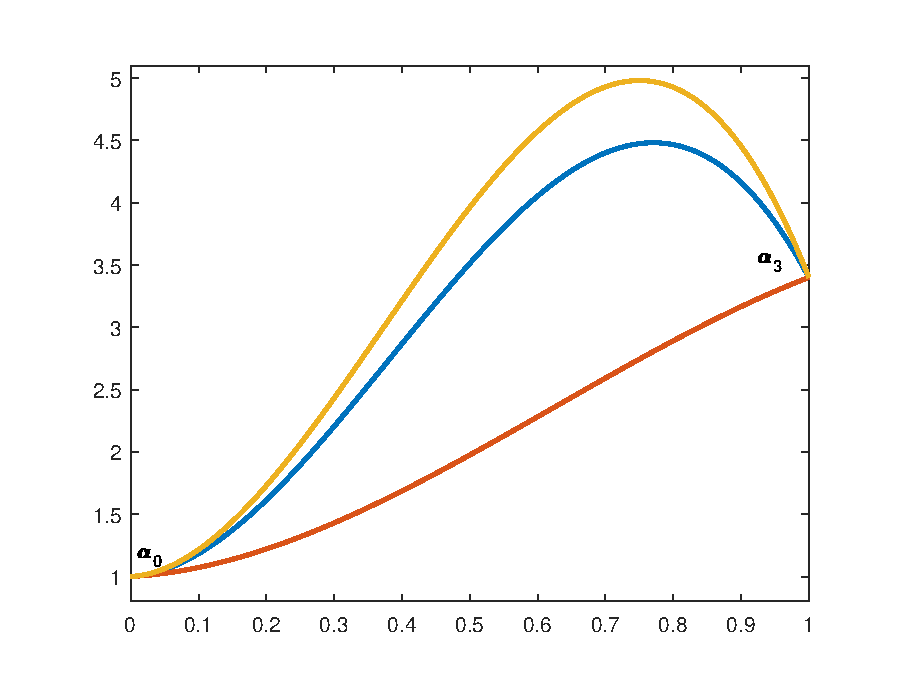
\includegraphics[width=.6\textwidth]{Images/bezier.eps}
\caption{Three bézier curve examples ($M = 4, \quad \alpha_0 = 1, \quad \alpha_{M-1} = 3.4$).}
\label{bezierPlot}
\end{figure}

This structure is very useful since the image of the polynomial is contained in the convex hull of the $M+1$ coefficients, viewed as points in $\mathbb{R}^2$. Moreover, it starts in $\alpha_0$ and it ends in $\alpha_M$ (but it does not pass through the other $\alpha_i$'s). The shape of the Bézier polynomials is also useful for numerical calculations, while computing the gradient of a cost functions to solve the optimization problem over the parameters $\alpha_i$'s. 

Once having defined such outputs, it is necessary to find the optimal numerical values of the parameters $\alpha_i$'s. This can be done, as already said, via trajectory optimization. So a cost function and several constraints must be defined. The goal in this work is to minimize the control energy, hence the cost function is straightforward
\begin{equation}
    J(\alpha) = \int_0^T\sum_{i=1}^{4}u_i^2(\alpha,t) dt
    \label{costFcn}
\end{equation}
where $u_i(t)$ is given by~\eqref{feedbackLinerizationControl}, and of course depends on the optimization parameters. 

In order to solve the optimization problem and simulate the locomotion of the five--link robot, a new MATLAB toolbox has been used, named FROST.

\subsection{FROST - Fast Robot Optimization and Simulation Toolkit}

FROST is an open--source toolbox for modeling, trajectory optimization and simulation of hybrid dynamical systems. The mathematical foundation of FROST is the feedback linearization technique, together with noninteracting control mentioned above.

\subsubsection{FROST Architecture}

\begin{figure}[H]
\centering
\includegraphics[width=.8\textwidth]{Images/FROSTFramework.PNG}
\caption{Block diagram of FROST architecture}
\label{blockdiagramfrostarch}
\end{figure}

As can be seen from \figurename~\ref{blockdiagramfrostarch}, the main feature of FROST is a custom symbolic toolbox (different from the standard one provided in MATLAB add--ons) which communicates with the kernel of Wolfram Mathematica. This approach allows to speed--up the computational time needed to complete all the operations, which can be very heavy if the robot has many degrees of freedom. Hence, all the kinematics and dynamics are computed in Wolfram starting from an Universal Robot Description Format (URDF)  file. Moreover, all the computations involving the trajectory optimization are performed in backend using powerful nonlinear programming solvers, like IPOPT or SNOPT.

\subsubsection{Hybrid Dynamical System in FROST}

The first feature of FROST is the definition of an abstract hybrid dynamical system, i.e. a system that presents both continuous and discrete dynamics. This fits perfectly with legged locomotion, which consists of a collection of continuous phases linked by discrete event triggering the passage from the phase $i$ to phase $i+1$.

In FROST, a hybrid system is a tuple
\begin{equation}
    \mathscr{HS} = (\Gamma, \mathcal{D}, \mathcal{U}, S, \Delta, C)
    \label{tupleHS}
\end{equation}
where $\Gamma = \{V,E\}$ is a directed graph composed by a set of vertices $V$ which represents the continuous phases and a set of edges $E$ that represents discrete events, $\mathcal{D}$ is the admissible configuration of the continuous domain, $\mathcal{U}$ represents the admissible controllers, $S$ determines the conditions that trigger discrete transitions, $\Delta$ and $C$ represent the discrete and the continuous dynamics, respectively. Note that the graph can be either cyclic or acyclic, depending on the application.

FROST uses the class \verb!ContinousDynamics! to represent a generic dynamical system of the type~\eqref{system}. This means that one can describe the dynamics of any biped robot using the Euler--Lagrangian formulation (see~\eqref{extModel}). On the other hand, by using the class \verb!DiscreteDynamics!, it is possible to characterize the instantaneous change from one phase into the other, i.e. when the swing foot of the robot hits the ground. To do this, it is necessary to specify:
\begin{enumerate}
    \item the event condition that triggers the change (swing foot vertical height equal to zero);
    \item a reset map, which is the mathematical formulation of the change
    \begin{equation}
        x^+ = \Delta_x(x^-)
    \end{equation}
    where $x$ is the state of the dynamical system, so including positions and velocity ($x = [q, \dot{q}]$), $x^- = \lim_{t\rightarrow{t_0^-}}x(t)$ and $x^+ = \lim_{t\rightarrow{t_0^+}}x(t)$, being $t_0$ the time instant at which the discrete dynamics occurs
\end{enumerate}

A hybrid system is generally constrained, so FROST provides a way to include the constraints in the model, essentially in two ways:
\begin{enumerate}
    \item \textbf{Holonomic Constraints.} FROST currently only supports holonomic constraints given as $h_c(x) = \textup{constant}$. These constraints are imposed via enforcing the second derivative of $h_c(x)$ to be zero, i.e.
    \[
    J_c(x)\ddot{x} + \dot{J}_c(x,\dot{x})\dot{x} = 0
    \]
    \item \textbf{Unilateral Constraints.} In order to specify complementarity condition during the contact with the ground, or other properties that the states or the inputs must have (e.g. saturation of actuators), FROST uses the class \verb!UnilateralConstraints! to introduce inequality constraints of the type 
    \[
    \mu(\cdot) \leq 0
    \]
    Differently from the holonomic ones, the unilateral constraints are not part of the simulation, but are considered as constraints in the optimization problem for determining the control law.
\end{enumerate}

As already said, FROST automatically build the kinematics and the dynamics of a robot once provided a URDF file. Currently, FROST supports just the description of joints, links and transmissions.

\subsubsection{Virtual constraints and feedback linearization control}

The main feature of this toolbox is the possibility to define the so--called \textit{Virtual Constraint}. A virtual constraint is defined via imposing that the difference between the actual output and the desired one is zero. This definition fits perfectly with the structure of the output~\eqref{systemOutput}. In fact, what FROST does in this case, is to enforce a constraint on the system output $y = h(q)$ during the optimization process. This is done using classical feedback linearization control to drive $y \rightarrow 0$. The controller has the form~\eqref{feedbackLinerizationControl}. It is important to note that, in order to define such a controller, one needs to perform the inversion of the decoupling matrix, which in the case of an underactuated five--link robot is a $4 \times 4$ matrix. Using a parameterized output with Bézier polynomials, this matrix will depend also on $\bm{\alpha}$, and so the computational effort needed to compute its inverse can be very high and not manageable using just the Symbolic Math Toolbox of MATLAB. On the contrary, FROST uses the kernel of Wolfram Mathematica, speeding up these calculations.

Once having performed the feedback linearization control, one can use the external control $v$ to impose the desired behaviour as in~\eqref{externalInput}.

\subsubsection{Hybrid Trajectory Optimization}

When one has built both a hybrid system and virtual constraints, FROST automatically sets up a nonlinear programming problem divided into different phases, depending on the hybrid definition of the system. In a very straightforward way, the cost function is defined over all the $N_p$ phases involved into the simulation
\begin{equation}
    J(\cdot) = \sum_{j=1}^{N_p} \int_{t_i^j}^{t_f^j} L_j(\cdot) dt.
    \label{FROSTcostfcn}
\end{equation}
where $L_j(\cdot)$ is the running cost of each phase. The cost $J(\cdot)$ is subject to the systems dynamics, the unilateral, holonomic and virtual constraints. The optimization problem can be at the end solved using, for instance, IPOPT, but also other NLP commercial solvers. If the solver is able to find an optimal solution, the final simulation can be done. The trajectory imposed to the robot can be visualized by 3D animators via RViz or by a custom stick animator in MATLAB environment.

\subsection{Simulation}

The toolbox FROST has been used in order to apply the feedback linearization and optimization control theory to the robot RABBIT. The actual output $h^a(q)$ is chosen simply as the femurs and tibias joint positions
\[
h^a(q) = 
\begin{bmatrix}
q_{31} \\
q_{32} \\
q_{41} \\
q_{42}
\end{bmatrix}.
\]
The degree of the Bézier polynomials is $M = 6$, which means that there are 28 parameters $\alpha_i$'s to be optimized. The optimization process, made with IPOPT, took about 12 [s] on a PC with an Intel i7, 2 GHz CPU and 8 GB RAM. A previous work~\cite{westervelt}, in which DIRCOL (another optimization toolbox) was used, indicates that the optimization time was much larger (about 21 minutes). 

In the simulation, one step lasts 0.5 [s] and the distance between the two feet during the double support phase is constant and equal to 0.37 [m]. In this section the control effort is reported: the actuators are equipped with a gearbox, whose ratio is $\tau = 50$. The torques depicted in \figurename~\ref{torque} are intended as those after the gearbox. The analysis of the trajectory and the velocity of the states will be done in section five, together with the analogous data retrieved from the next approach, i.e. the gait generation via differential kinematics.

\begin{figure}[H]
\centering
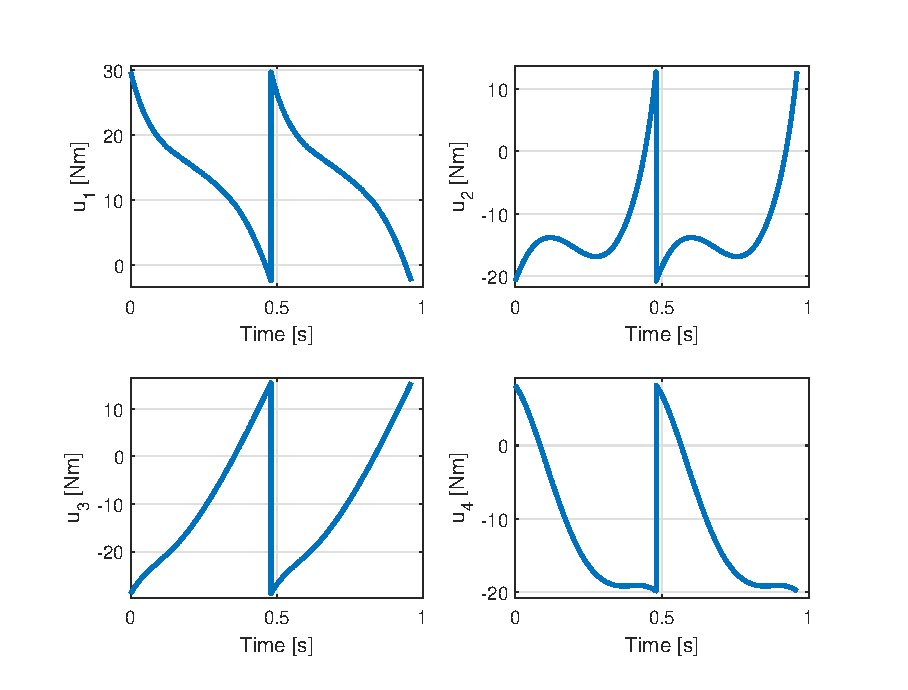
\includegraphics[width=.8\textwidth]{Images/torques.eps}
\caption{Torque curves for two steps}
\label{torque}
\end{figure}

\section{Bounded CoM Trajectory Tracking}

In this second approach the gait for the humanoids has been generated by tracking a bounded CoM trajectory.

First, a simple model is exploited in order to approximate the robot dynamics. This will be the Linear Inverted Pendulum (LIP) model, which relates the center of mass acceleration to an external input suitably defined. This model is unstable but by ensuring some conditions on the initial state, the boundedness of the system evolution can be guaranteed.

For the control design, instead, a simple ZMP step trajectory will be defined and this will be the input to the LIP model. Then, a stable CoM trajectory will be generated by simulating the LIP model and finally the tracking of this trajectory will be executed using the differential kinematics of the robot, by also including additional tasks which are essential for the generation of the humanoid gait.

\subsection{Linear Inverted Pendulum}

As already said, an effective approximation of the Robot dynamics for control purposes is the LIP model. The dynamics of this system in the sagittal plane is defined in the following way
\begin{equation}
\label{eqn:complete_lip_model}
\ddot{x}_c = \frac{g}{h_o}(x_c-x_a)+\frac{1}{mh_o}(\tau_a-\tau_h)+\frac{F(t)}{m}
\end{equation}
with $x_a$ the point foot location, $x_c$ the CoM horizonta position, $h_o$ its constant heigth, $m$ its centered mass, $\tau_a$ an ankle torque and $\tau_h$ a hip torque acting on a reaction mass.

Moreover, defining $\omega_o = \sqrt{\dfrac{g}{h_o}}$ and including in the term $z(t)$ all external inputs, including possible disturbances, the equation (\ref{eqn:complete_lip_model}) can be rewritten as
\begin{equation}
\label{eqn:general_lip_model}
\ddot{x}_c = \omega_o^2x_c(t) - \omega_o^2z(t)
\end{equation}
By looking at the RABBIT system, though, some other simplifications can be inferred on the model.

The case study robot, in fact, has point foots. Therefore, it can be assumed that there are no ankle torque $\tau_a$ and hip torque $\tau_h$. Moreover, the pendulum can be seen as a massless telescoping leg with point foot location in $x_a$ and a point mass $m$ kept at constant height $h_o$.

The Zero Moment Point (ZMP), the point around which the moment of the ground reaction forces is null, and the Center of Pressure (CoP), the application point of the resultant of the ground reaction forces, coincide and they are fixed in $x_a$ if no step is taken. From this, it can be concluded that $x_a$ can be considered as a control input $z(t)$ and in the absence of external disturbances the dynamics (\ref{eqn:complete_lip_model}) is simply
\begin{equation}
\label{eqn:point_foot_model}
\ddot{x}_c = \omega_o^2x_c(t) - \omega_o^2x_a.
\end{equation}
Finally it will be helpful for later discussion to represent the system in state-space form, taking as state $(x_c,\dot{x}_c)$, whose equations are
\begin{equation}
\label{eqn:lip_state_space}
\begin{pmatrix}
\dot{x}_c\\
\ddot{x}_c
\end{pmatrix}=\begin{pmatrix}
0 & 1\\
\omega_o^2 & 0
\end{pmatrix}\begin{pmatrix}
x_c \\
\dot{x}_c
\end{pmatrix}+\begin{pmatrix}
0 \\
-\omega_o^2
\end{pmatrix}z(t).
\end{equation}

\subsection{Bounded Solutions For LIP Model}

Under the explained approximation, the relationship between the ZMP and the CoM is governed by an unstable second order system.

This can be easily shown by applying a change of coordinates
\begin{equation}
\label{eqn:change_coordinates}
\begin{pmatrix}
x_u\\
x_s
\end{pmatrix}=\begin{pmatrix}
1 & 1/\omega_o\\
1 & -1/\omega_o^2
\end{pmatrix}\begin{pmatrix}
x_c \\
\dot{x}_c
\end{pmatrix}
\end{equation}
and decouple the stable and unstable dynamics
\begin{equation}
\label{eqn:change_coordinates_dynamics}
\begin{pmatrix}
\dot{x}_u\\
\dot{x}_s
\end{pmatrix}=\begin{pmatrix}
\omega_o & 0\\
0 & -\omega_o
\end{pmatrix}\begin{pmatrix}
x_u \\
x_s
\end{pmatrix}+\begin{pmatrix}
-\omega_o \\
\omega_o
\end{pmatrix}z(t)
\end{equation}
from which it is possible to notice that unstable dynamics is due to the dynamics of $x_u$ whose evolution is determined by the positive eigenvalue $+\omega_o$.

The aim, now, is to be able to select trajectories of the system that remain bounded and avoid the divergent behaviour associated to eigenvalue $+\omega_o$. This can be achieved either by choosing a particular initial condition $x_u(t_0)$, or by designing the input $z(t)$ to mantain $x_u(t)$ bounded.

\subsubsection{Unstable Subsystem}

By looking at the first row of the system (\ref{eqn:change_coordinates_dynamics}), the solution of the $x_u$ dynamics is given by
\begin{equation}
\label{eqn:x_u_solution}
x_u(t;z) = e^{\omega_o(t-t_0)}x_u(t_0)-\omega_o\int_{t_0}^t{e^{\omega_o(t-\tau)}z(\tau)d\tau}
\end{equation}
In general this solution diverges, however if the initial condition satisfies
\begin{equation}
\label{eqn:x_u_general_init}
x_u(t_0) = x_u^*(t_0;z) = \omega_o\int_{t_0}^\infty{e^{-\omega_o(\tau-t_0)}z(\tau)d\tau}
\end{equation}
the evolution becomes
\begin{equation}
\label{eqn:x_u_bounded_ev}
x_u^*(t;z) = \omega_o\int_{0}^\infty{e^{-\omega_o\tau}z(\tau+t)d\tau}
\end{equation}
which is bounded under some boundedness condition on the input $z(t)$.

It is important to notice that under the change of coordinates given by (\ref{eqn:change_coordinates}), the condition (\ref{eqn:x_u_general_init}) defines a constraint on the initial conditions for the center of mass trajectory, which can be called \textit{boundedness condition}
\begin{equation}
\label{eqn:boundedness_condition}
x_u^*(t_0;z) = x_c(t_0) + \frac{1}{\omega_o}\dot{x}_c(t_0).
\end{equation}
It will be essential in the the planning of stable CoM trajectories.

\subsection{Planning and Control Design}

As anticipated, the condition (\ref{eqn:boundedness_condition}) is essential to generate a stable CoM to be tracked. Since (\ref{eqn:boundedness_condition}) depends both on the input and the initial conditions of the CoM, it can be used either to infer constraints on the initial conditions when the input is defined or viceversa.

\subsubsection{Constraints on Initial Condition}

Supposing that $z(t)$ is defined, it is possible to directly compute $x_u^*(t_0;z)$ by evaluating (\ref{eqn:x_u_general_init}). Now (\ref{eqn:boundedness_condition}) defines a linear constraint between $x_c(t_0)$ and $\dot{x}_c(t_0)$ and so by fixing one of the two one can compute the other, by ensuring the boundedness of the CoM trajectory.

Assuming that $x_c(t_0)$ is specified, it holds
\begin{equation}
\label{eqn:init_vel}
\dot{x}_c(t_0) = \omega_o[x_u^*(t_0;z)-x_c(t_0)].
\end{equation}
Instead, assuming that $\dot{x}_c(t_0)$ is given, then the initial position will be
\begin{equation}
\label{eqn:init_pos}
x_c(t_0) = x_u^*(t_0;z) - \frac{1}{\omega_o}\dot{x}_c(t_0).
\end{equation}

\subsubsection{Constraints on Control Design}

Now, instead, the assumption is that both $x_c(t_0)$ and $\dot{x}_c(t_0)$ are given. Hence one can design the control input in such a way that the constraint (\ref{eqn:boundedness_condition}) is still satisfied. 

In particular, let us consider the case in which the system input is a linear combination of known functions $z_i$'s
\begin{equation}
\label{eqn:input_comb}
z(t) = \sum{\alpha_iz_i(t)}.
\end{equation}
For example, the $z_i$'s could be a collection of step functions, cubic splines or monotonic functions. For this class of of inputs, it is possible to rewrite (\ref{eqn:boundedness_condition}) to infer constraints on the choice of the design parameters $\alpha_i$. Indeed, using the linearity of $z(t)$ in (\ref{eqn:x_u_solution}) and taking the input train as a series of step, each one occurring at fixed time $t_i$, one can write
\begin{equation}
\label{eqn:x_u_init_z_comb}
x_u(t_0) = x_u^*(t_0;z) = \sum_i{\alpha_ix_u^*(t_0;z_i)} = \sum_i{\alpha_i e^{-\omega_o t_i}}.
\end{equation}
Therefore (\ref{eqn:x_u_init_z_comb}) defines a linear constraint on the $\alpha_i$. Given a sufficient number of other constraints one may solve uniquely for the $\alpha_i$'s, otherwise one could choose the parameters by optimizing some criteria.

For example if one has a single input, then by imposing the condition (\ref{eqn:boundedness_condition}) $\alpha$ is fixed:
\[
\begin{split}
\alpha x_u^*(0;z) & = x_c(0) + \frac{1}{\omega_o}\dot{x}_c(0)\\
\alpha & = \frac{1}{x_u^*(0;z)}[x_c(0) + \frac{1}{\omega_o}\dot{x}_c(0)]
\end{split}.
\]

\subsection{CoM Trajectory in RABBIT}

Now the results obtained in the generation of a suitable CoM trajectory in the case study of the RABBIT robot model are reported.

Considering the case of a single step, a normalized step function has been chosen as reference input, represented by the Heaviside function, with the control design parameter $\alpha$ representing the amplitude of the step and $t_a$ the instant at which the step is taken:
\begin{equation}
\label{eqn:step_funct}
z(t) = \alpha z_{step}(t-t_a).
\end{equation}
Since the input to the LIP model is the point foot, this is equivalent to say that the $x$ coordinate of the stance point foot remains fixed to its position up to the point when the swing leg touches the ground. In that instant, the swing leg becomes the new stance leg and therefore the stance point foot has a jump in its value, since it is instantaneously moved forward.

For this particular input the initial condition for the unstable dynamics of the LIP model is quite simple to compute, so the equation (\ref{eqn:x_u_general_init}) becomes
\begin{equation}
\label{eqn:step_x_u_init}
x_u(t_0) = x_u^*(t_0;z) = \omega_o\int_{0}^\infty{e^{-\omega_o(\tau-t_0)}z(\tau)d\tau} = e^{-\omega_ot_a}.
\end{equation}

In the experiment the value of $\alpha$ has been fixed. Moreover, since it could be useful for the comparison, the initial configuration has been chosen to be equal to the one of FROST simulation. With this setting, then, $\dot{x}_c(t_0)$ is obliged to be (\ref{eqn:init_vel})
\begin{equation}
\label{eqn:init_vel_rabbit}
\dot{x}_c(t_0) = \omega_o[e^{-\omega_ot_a}-x_c(t_0)].
\end{equation}
After having found all the initial conditions, in order to generate the CoM trajectory, the evolution of the system has been simulated (\ref{eqn:change_coordinates_dynamics}) by computing $x_u(0)$ using the change of coordinates. The outputs of the system are $x_c$ and $\dot{x}_c$ whose dependencies from the state can be retrieved by inverting the change of coordinates transformation
\begin{equation}
\label{eqn:com_wrt_change}
x_c = \frac{1}{2}(x_u+x_s) \quad \quad \dot{x}_c = \frac{\omega_o}{2}(x_u-x_s)
\end{equation}
With CoM intial condition $x_c(0) = -0.168$, the duration of a time step equals to 1 second and amplitude $\alpha = 0.37$, the CoM trajectory and velocity, considering the case of two steps, are the following:

\begin{figure}[H]
\centering
\subfloat[][CoM Trajectory]{
\includegraphics[width=.4\linewidth]{Images/com_traj.eps}
\label{fig:com_trajectory}
}
\subfloat[][CoM Velocity]{
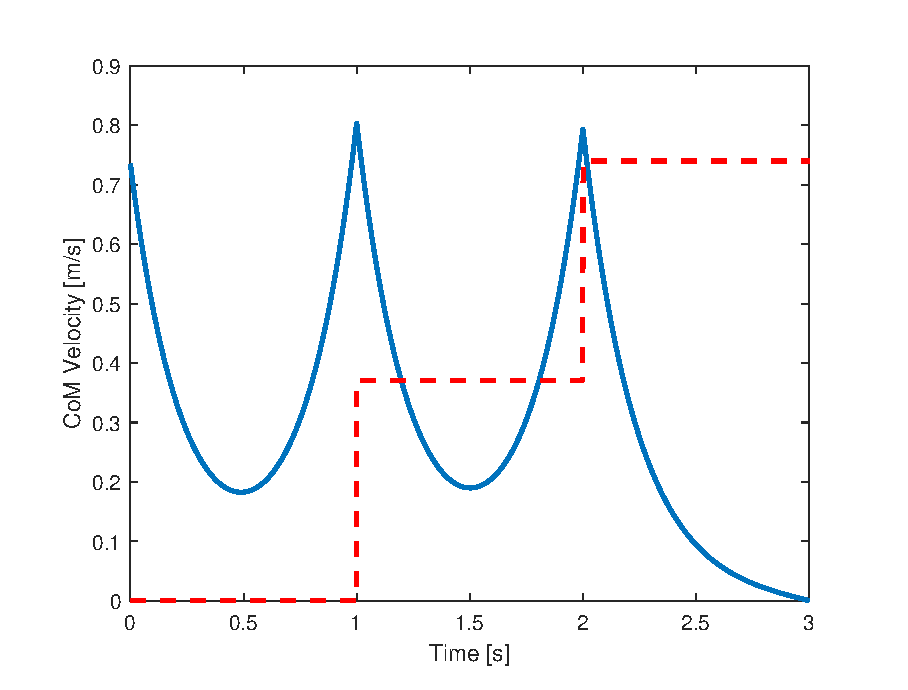
\includegraphics[width=.4\linewidth]{Images/com_vel.eps}
\label{fig:com_vel}
}
\caption{CoM Trajectory and Velocity}
\end{figure}
It is important to notice that the generated motion is almost periodic and therefore the general strategy for the simulation will be to track the trajectory only during the duration of a single step. In this way one obtains joint coordinates that after two steps repeat themselves and can assign the correct values by switching the order of the joint in the swing and stance leg.

\subsection{CoM Tracking in RABBIT}

Once generated the CoM trajectory, the robot needs to execute it. A simple way to achieve this is through kinematic tracking. The tasks to be executed must be defined and, working on velocities, the joint commands must be retrieved.

First, it is important to remember that the model is planar and lies in the plane defined by the axis $(x,z)$, therefore all the position tasks will be simply 2--dimensional.

The tasks are defined in the following way:

\begin{itemize}
\item \textbf{CoM Position}: in this case the $x$ and $\dot{x}$ trajectory were computed in the previous section, while the $z$ coordinates needs to remain at a fixed value $h_o$ for the model assumption, so its velocity will be 0
\begin{equation}
\label{eqn:com_task}
c_d = \begin{pmatrix}
x_c \\
h_o
\end{pmatrix} \quad \dot{c}_d = \begin{pmatrix}
\dot{x}_c \\
0
\end{pmatrix}.
\end{equation}
Now the direct kinematics of the robot links the CoM position w.r.t. the joints coordinates $c=p_1(q)$ which actually depends only on the stance leg coordinates. Assuming the same gait considerations made in the previous section, the task profiles are
\begin{figure}[H]
\centering
\subfloat[][CoM x coordinate Trajectory]{
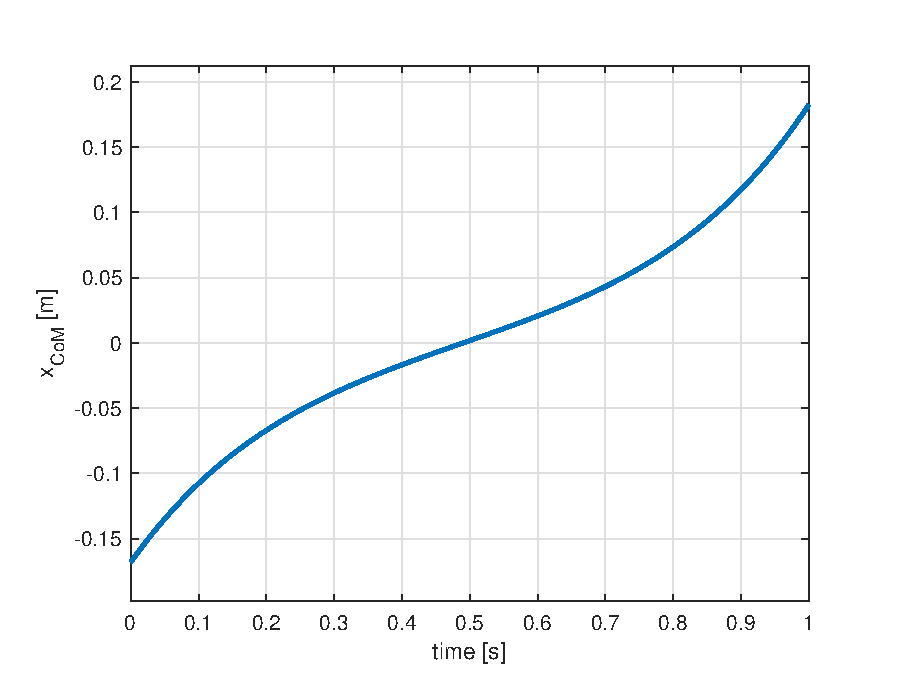
\includegraphics[width=.4\linewidth]{Images/com_x_pos.eps}
\label{fig:traj_1}
}
\subfloat[][CoM x coordinate Velocity]{
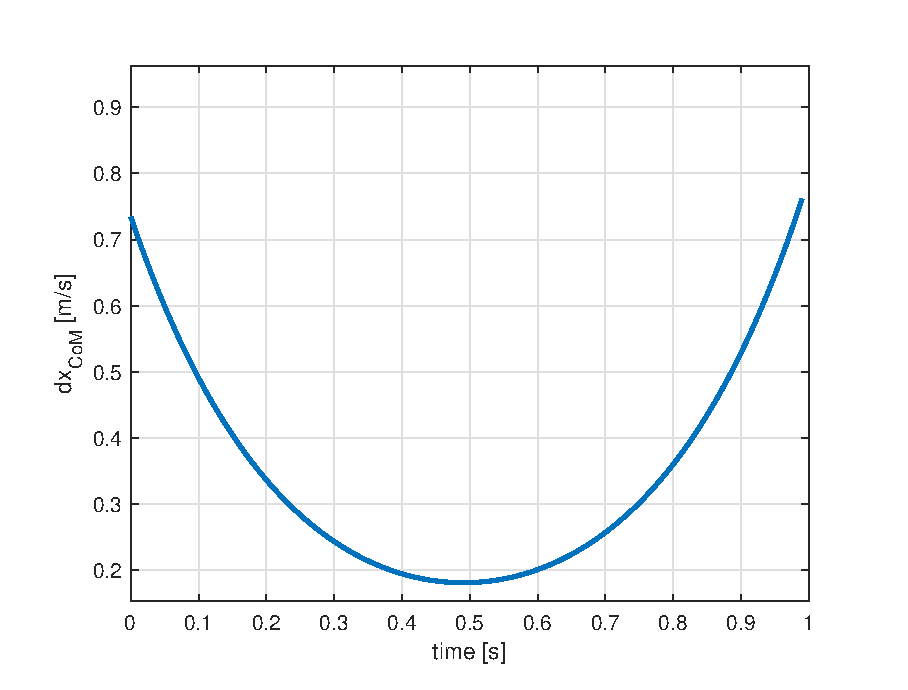
\includegraphics[width=.4\linewidth]{Images/com_x_vel.eps}
\label{fig:vel_1}
}
\caption{CoM Task}
\end{figure}
\item \textbf{Torso Orientation}: without this task the robot leaned too forward during the gaits. Therefore, a trajectory for the orientation of the torso has been built. In particular, the orientation of the FROST experiment during the gait has been taken as a reference, by using interpolation to derive a suitable profile to be tracked in the simulation
\begin{equation}
\label{eqn:com_or_task}
\theta_d = \theta_y \quad \dot{\theta}_d = \dot{\theta}_y.
\end{equation}
Since the environment is planar, the orientation of the CoM is only around the $y$ axis and the direct kinematics is simply given by the first joint coordinate $\theta=q_1$. Considering the step duration equals to 1 second, the generated profile are
\begin{figure}[H]
\centering
\subfloat[][Trajectory of Torso Orientation]{
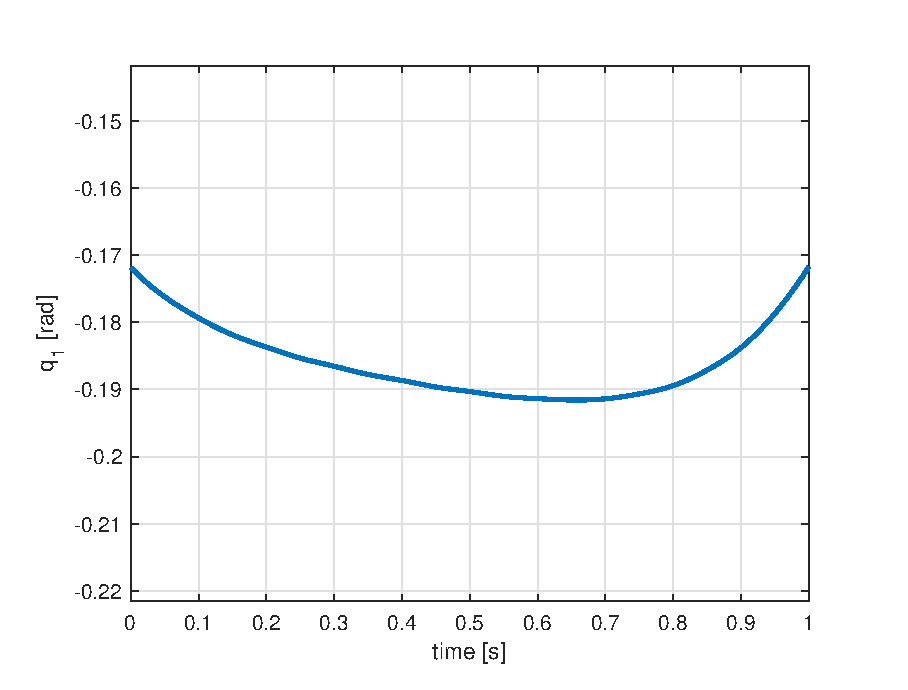
\includegraphics[width=.4\linewidth]{Images/torso_pos.eps}
\label{fig:traj_3}
}
\subfloat[][Velocity of Torso Orientation]{
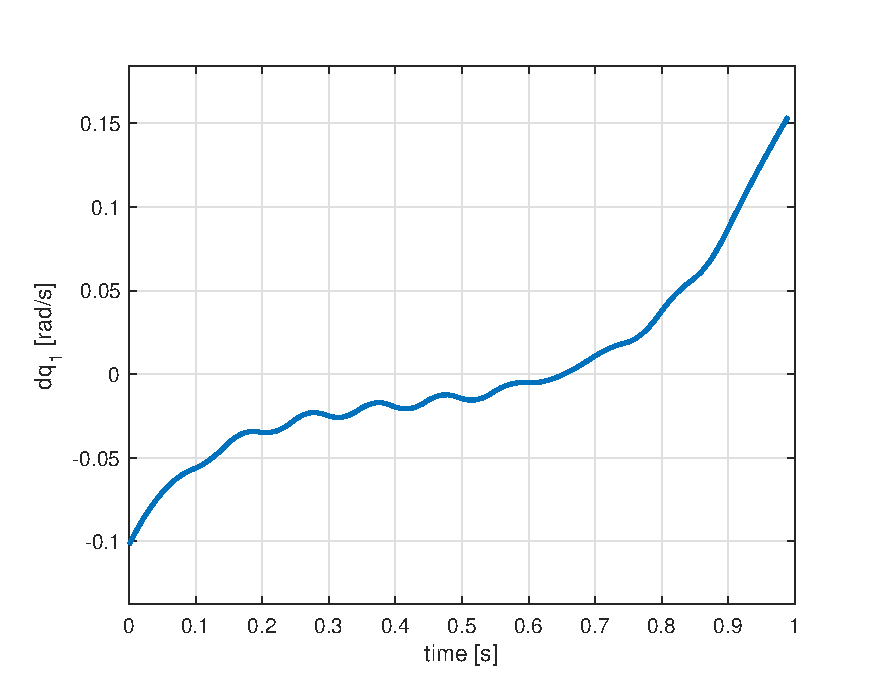
\includegraphics[width=.4\linewidth]{Images/torso_vel.eps}
\label{fig:vel_3}
}
\caption{Torso Task}
\end{figure}
\item \textbf{Swing Foot Position}: Since the position of the CoM actually depends only on the joint variables of the stance leg, another task is needed in order to derive suitable joint values for the swing leg during the gait. In order to generate this task, two different trajectories have been built for the $x$ and $z$ coordinates of the swing foot. For the $x$ coordinate a linear profile has been chosen. For the $z$ coordinate, instead, a parabola has been taken: its value is $0$ at the start and at the end of the step and reaches a predefined maximum value $z_{max}$
\begin{equation}
\label{eqn:sf_traj}
x_{sf}(t) = x_{sf}(t_0) + p(t)(x_{sf}(t_f)-x_{sf}(t_0)) \quad z_{sf}(t) = -\frac{4z_{max}}{t_f^2}t(t-t_f)
\end{equation}
\begin{equation}
\label{eqn:sf_task}
f_d = \begin{pmatrix}
x_{sf} \\
z_{sf}
\end{pmatrix} \quad \dot{f}_d = \begin{pmatrix}
\dot{x}_{sf} \\
\dot{z}_{sf}
\end{pmatrix}.
\end{equation}
Now, via the direct kinematics of the robot, one can express the swing foot position w.r.t. the joints coordinates $f=p_2(q)$ which actually depends only on the swing leg coordinates.\\
Assuming that the duration of a single step is 1 second the profiles for the two coordinates are the following
\begin{figure}[H]
\centering
\subfloat[][Swing Foot x coord.]{
\includegraphics[width=.4\linewidth]{Images/sw_x_pos.eps}
\label{fig:traj_4}
}
\subfloat[][Swing Foot x vel.]{
\includegraphics[width=.4\linewidth]{Images/sw_x_vel.eps}
\label{fig:vel_4}
}\\
\subfloat[][Swing Foot z coord.]{
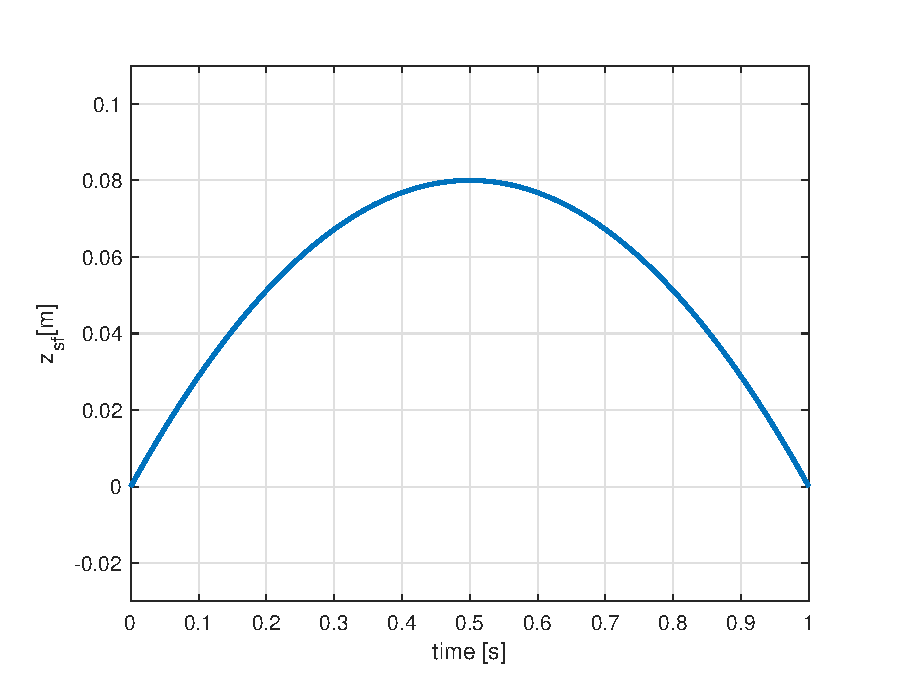
\includegraphics[width=.4\linewidth]{Images/sw_z_pos.eps}
\label{fig:traj_5}
}
\subfloat[][Swing Foot z vel.]{
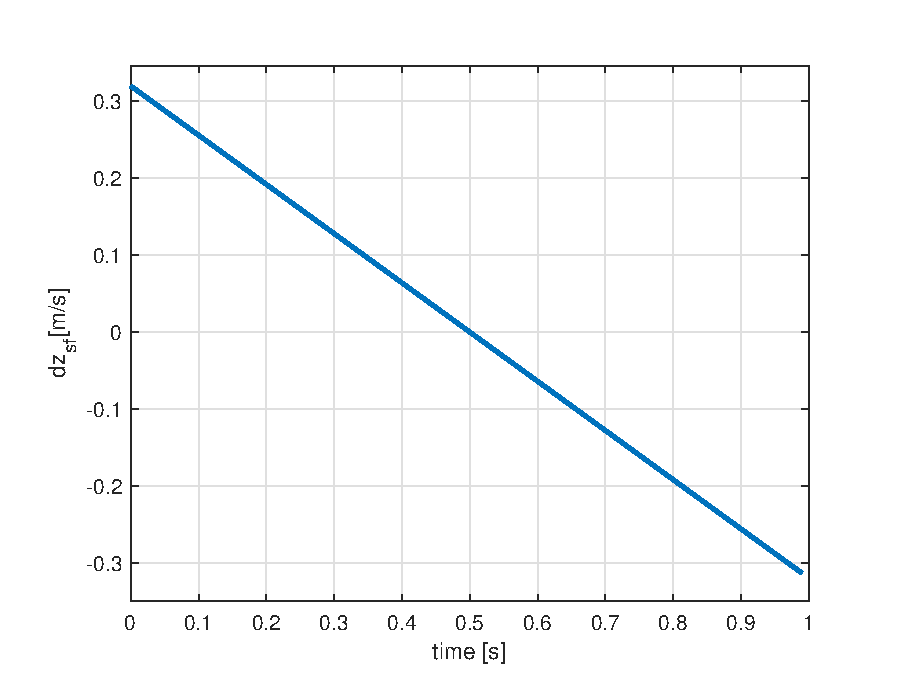
\includegraphics[width=.4\linewidth]{Images/sw_z_vel.eps}
\label{fig:vel_5}
}
\caption{Swing Foot Task}
\end{figure}
\end{itemize}

Now that all the tasks are defined, it is necessary to introduce the differential kinematics in order to generate joint commands to track the trajectories. After defining all the correct tasks Jacobians, the problem can be reformulated in the following way
\begin{equation}
\label{eqn:stack_of_tasks}
\dot{t} = \begin{pmatrix}
\dot{c}\\
\dot{\theta}\\
\dot{f}
\end{pmatrix} = \begin{pmatrix}
J_c(q)\\
J_{\theta}(q)\\
J_f(q)
\end{pmatrix}\dot{q} = J_t(q)\dot{q}.
\end{equation}
The solution can be simply found using the pseudoinverse of $J_t$ and adding a position error in order to avoid drifting in the tracking
\begin{equation}
\label{eqn:vel_command}
\dot{q} = J_t^\#(\dot{t}_d + k(t_d-t))
\end{equation}

Since the motion related to the gait is almost periodic, what one can actually do is to find the joint commands during the duration of a single step and then use the same commands at the next step but reordering the joint coordinates because stance leg and swing leg are switched. Note that the final configuration of the stance leg at the end of the step is almost coincident with the one of the swing leg when the step begins, so it is possible to switch the two profiles between them (see \figurename~\ref{2steps}). 

A simple MATLAB algorithm to find the joint coordinates is now reported:

\begin{Verbatim}[tabsize = 4, frame = lines, numbers = left]
com_ref = [x_c';z_c'];
stack_pos = [com_ref;q_torso_ref(1:end-1);swing_ref(:,1:end-1)];
com_vel = [x_c_dot';z_c_dot'];
stack_vel = [com_vel;q_torso_dot_ref;swing_vel];

stack_num = zeros(5,Tf+1);

for i=1:Tf
    j_num = single(subs(jac,q_sym,q_actual'));
    stack_num(:,i) = single(subs(dir_kin,q_sym,q_actual'));
    q_dot(:,i) = j_num \ (stack_vel(:,i)+gain*(stack_pos(:,i) ...
    - stack_num(:,i)));
    q(:,i+1) = q(:,i) + deltaT*q_dot(:,i);
    q_actual = q(:,i+1);
end
\end{Verbatim}

For each instant in the duration of a single step, one creates the tasks stack needed. Then, the stacked Jacobian is evaluated and (\ref{eqn:vel_command}) is used to compute the joint velocities. Finally, the joints values are retrieved by simply integrating the joints velocities.

Considering the defined task and the step duration of 1 seconds with amplitude $\alpha = 0.37$, the obtained RABBIT generalized coordinates values and velocities during two steps are depicted.

\begin{figure}[H]
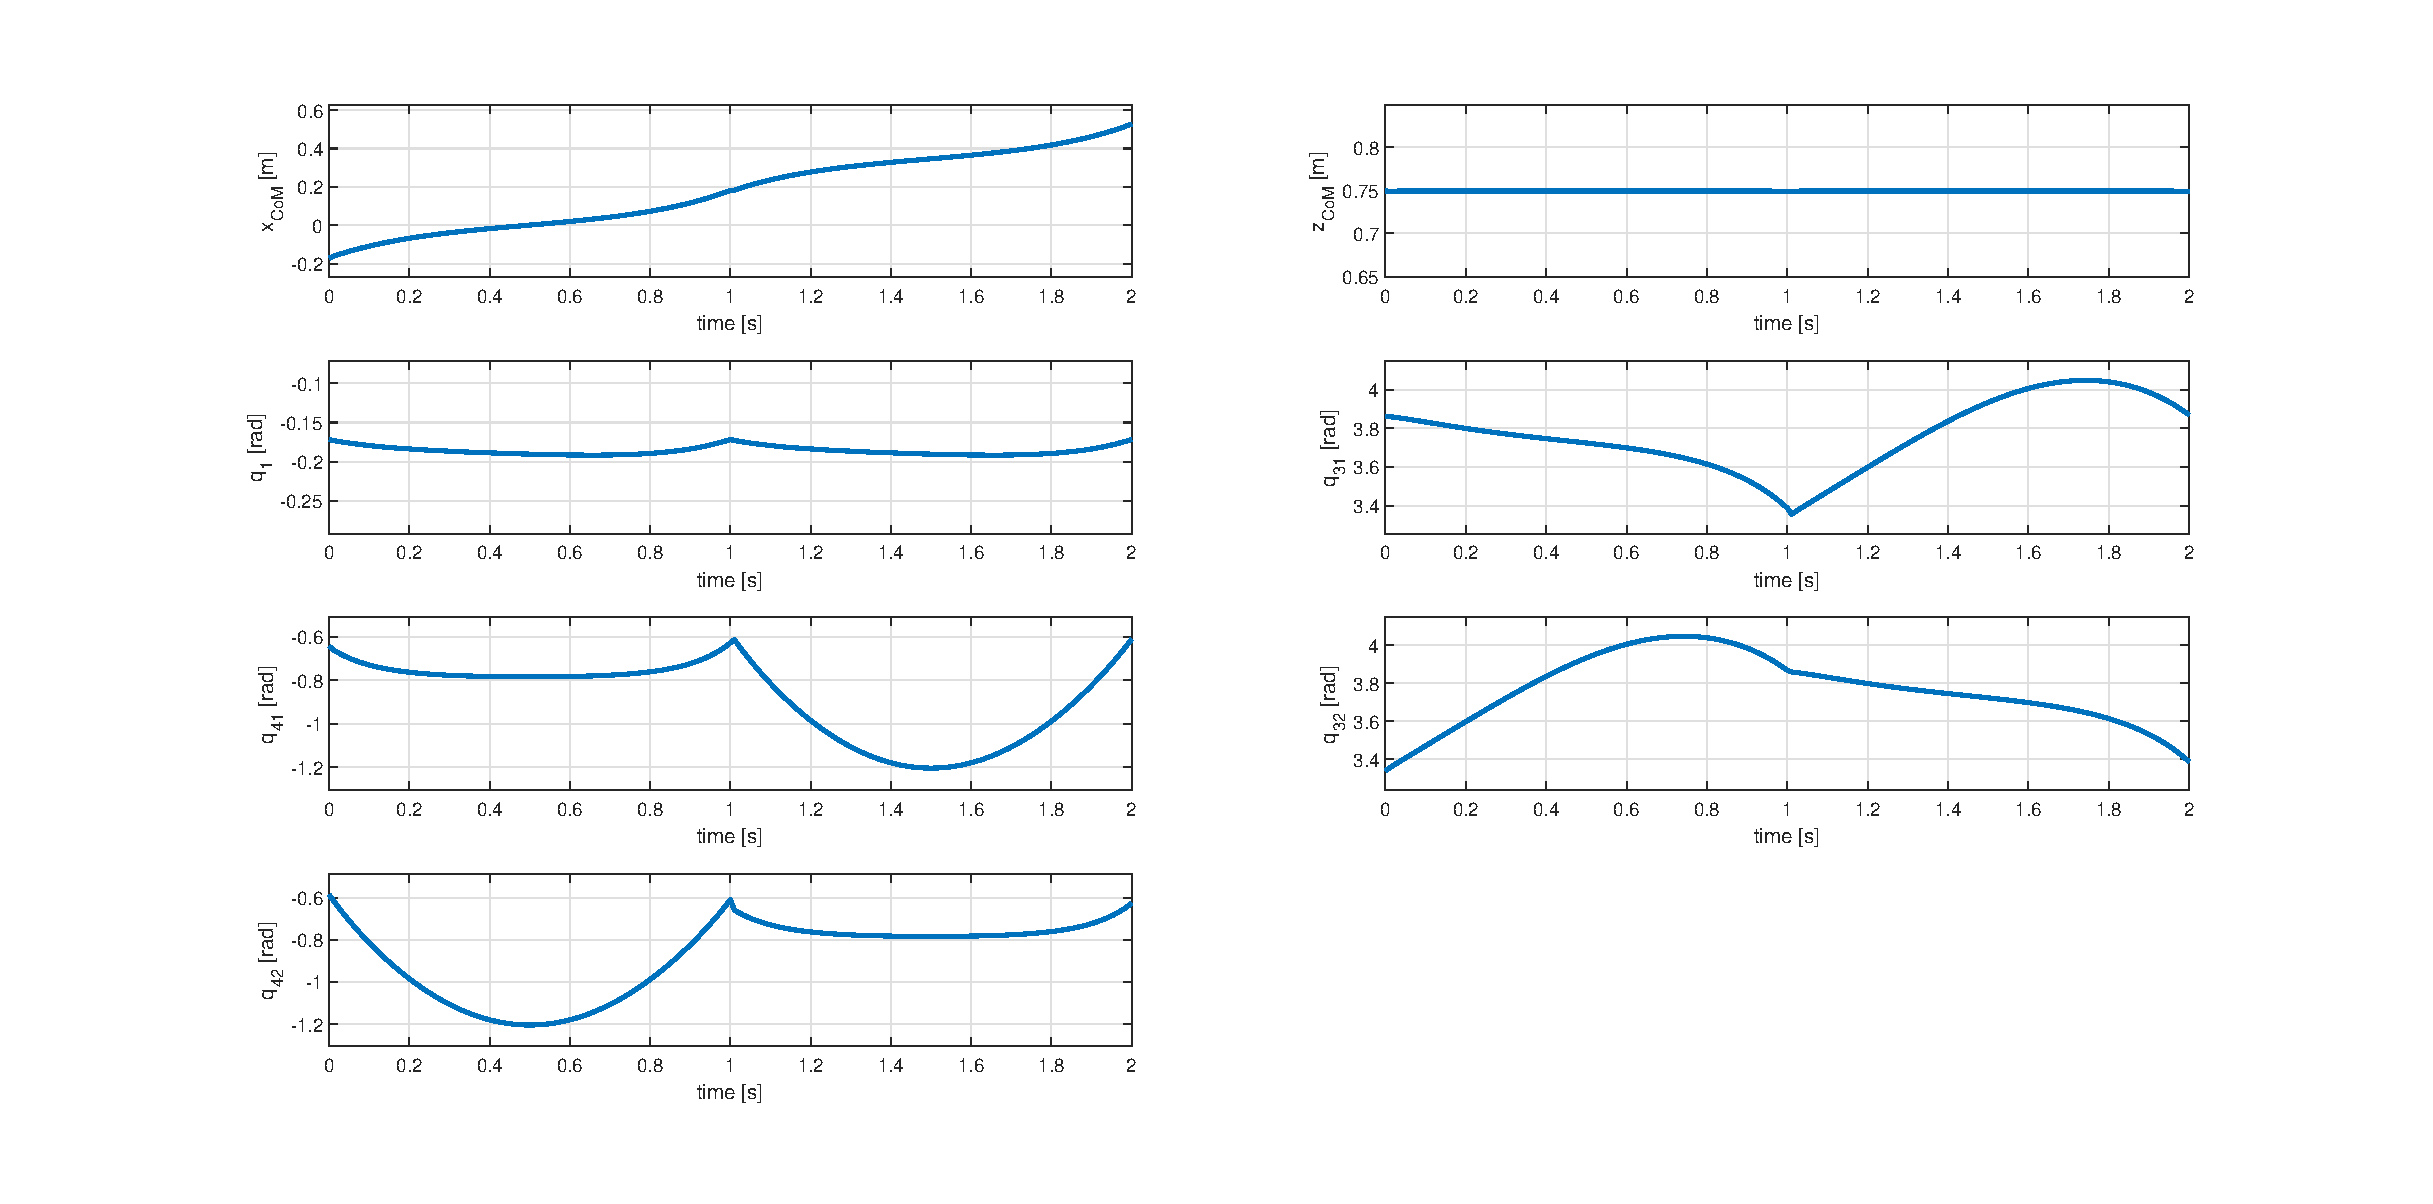
\includegraphics[width=1\linewidth]{Images/pos_2_steps_1_second.eps}
\caption{Generalized Coordinates 2 Steps}
\label{2steps}
\end{figure}

It is worth focusing on the initial stance leg joint coordinates $(q_{31},q_{41})$ and initial swing leg coordinates $(q_{32},q_{42})$. It is possible to see that after the step instant their roles are inverted and they simply follow the previous profiles of the other leg joints. So, in a certain way, the legs joints at the same level of the respective leg chains follow each other but with a delay equals to the step duration. Moreover, note that for each joint the motion is periodic (the period is twice the step duration), whereas at the step instant there is a continuity at the joints values but a discontinuity at the velocity level, as the impact model predicted. The last statement can be easily verified by reporting also the velocities of the generalized coordinates
\begin{figure}[H]
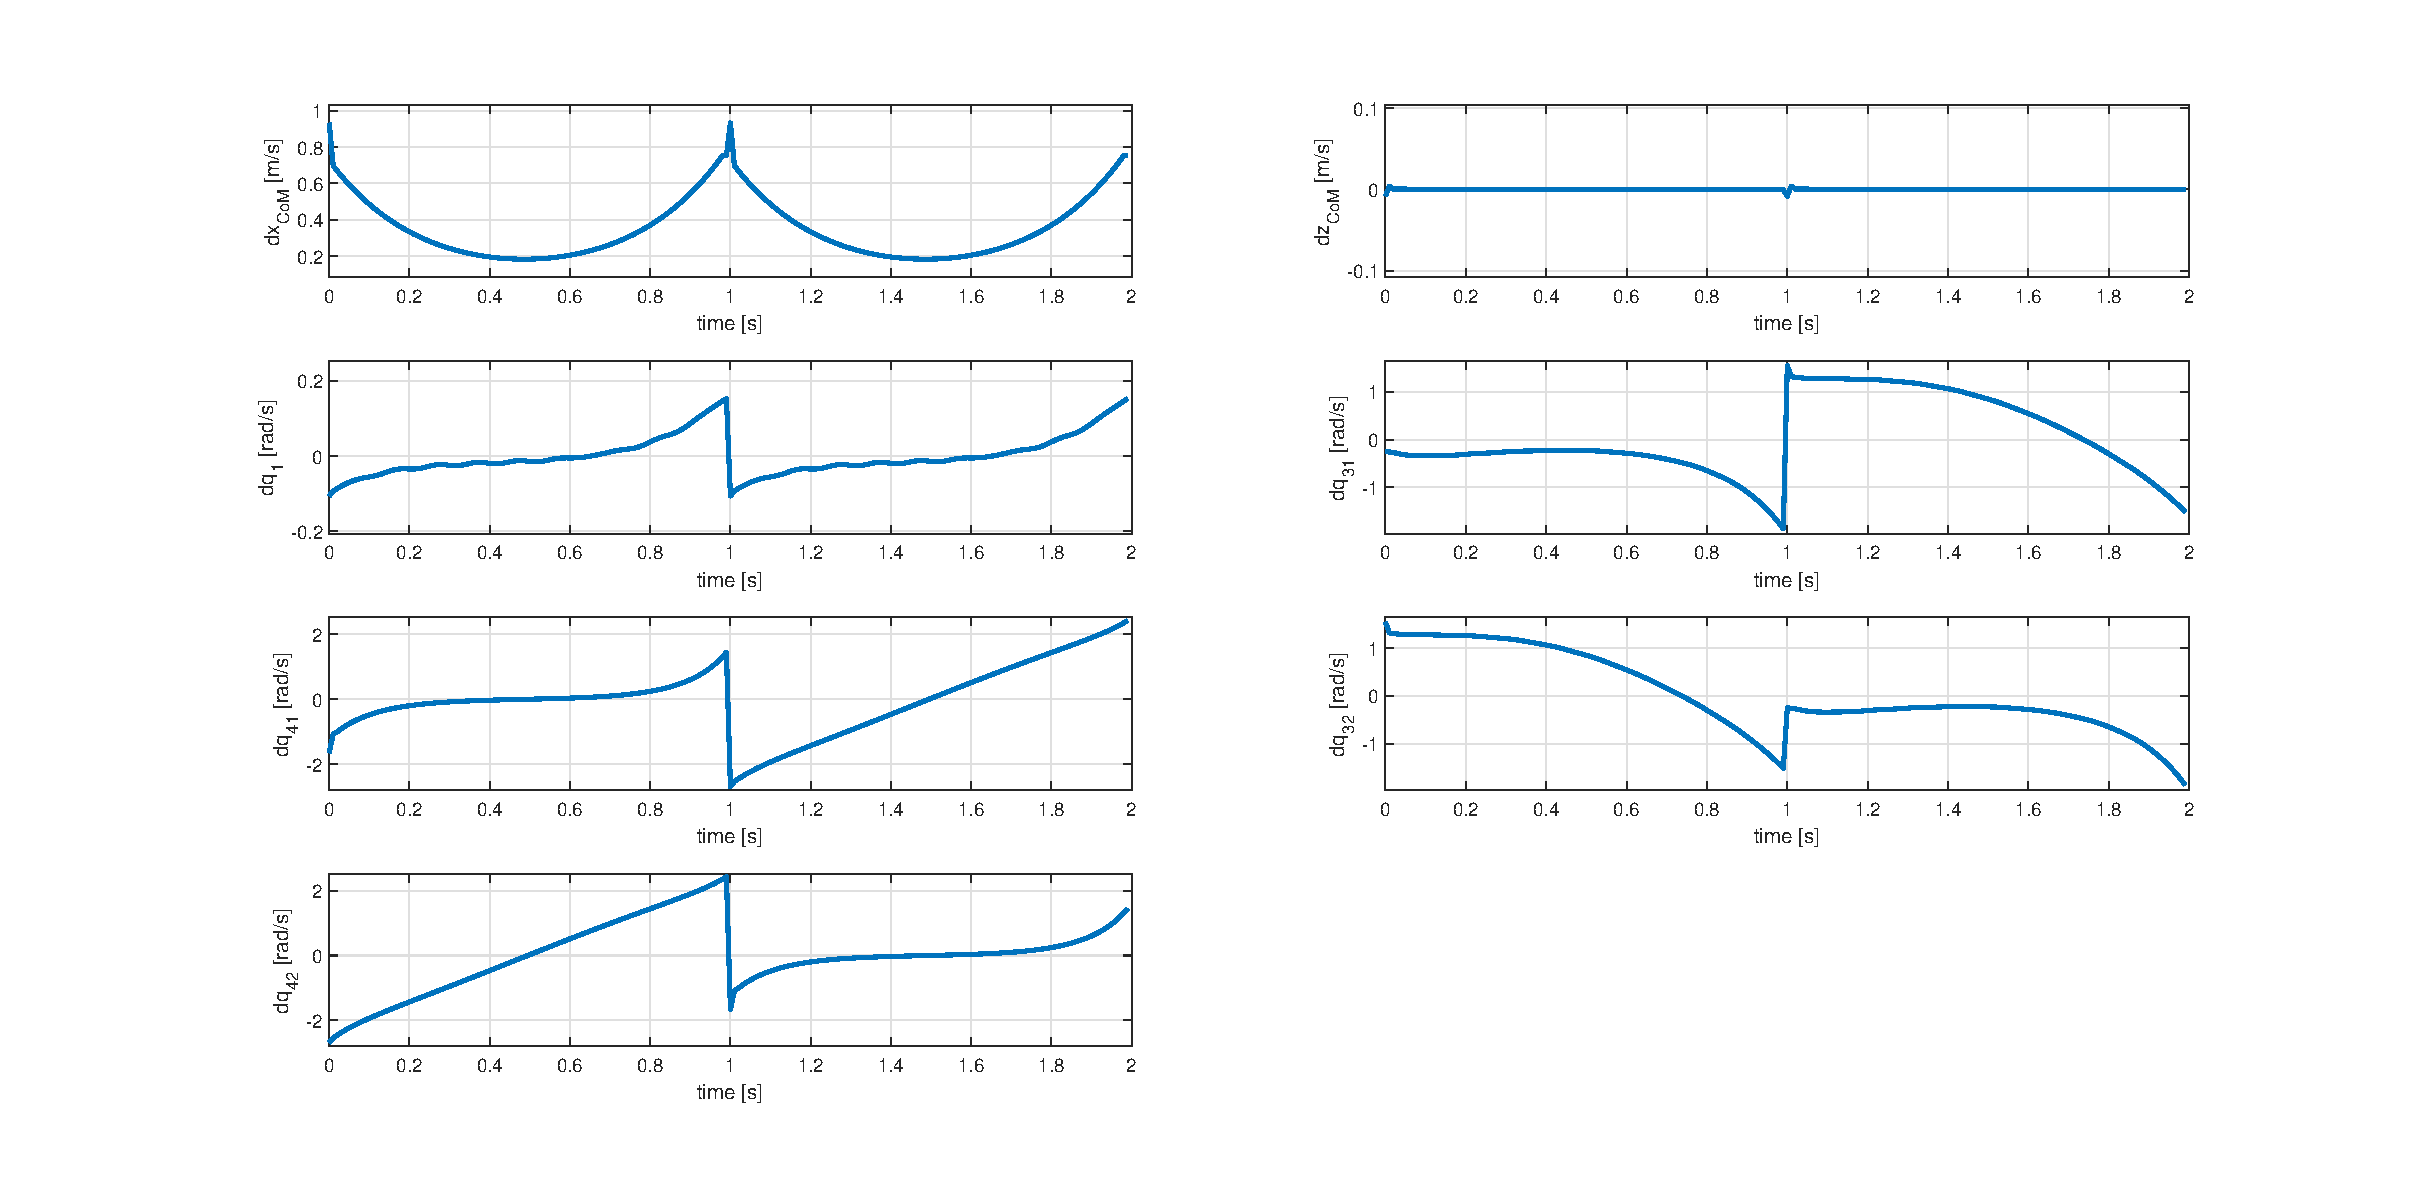
\includegraphics[width=1\linewidth]{Images/vel_2_steps_1_second.eps}
\label{fig:2_steps_1_second_vel}
\caption{Generalized Coordinates Velocity 2 Steps}
\end{figure}

Eventually, the results of the tracking of the tasks trajectories previously defined are shown. The gains for drifting recovery were set to $100$ and it is possible to note that the tracking is very accurate for this particular gait. The blue lines are the reference trajectories, whereas the red dashed lines are the executed ones.
\begin{figure}[H]
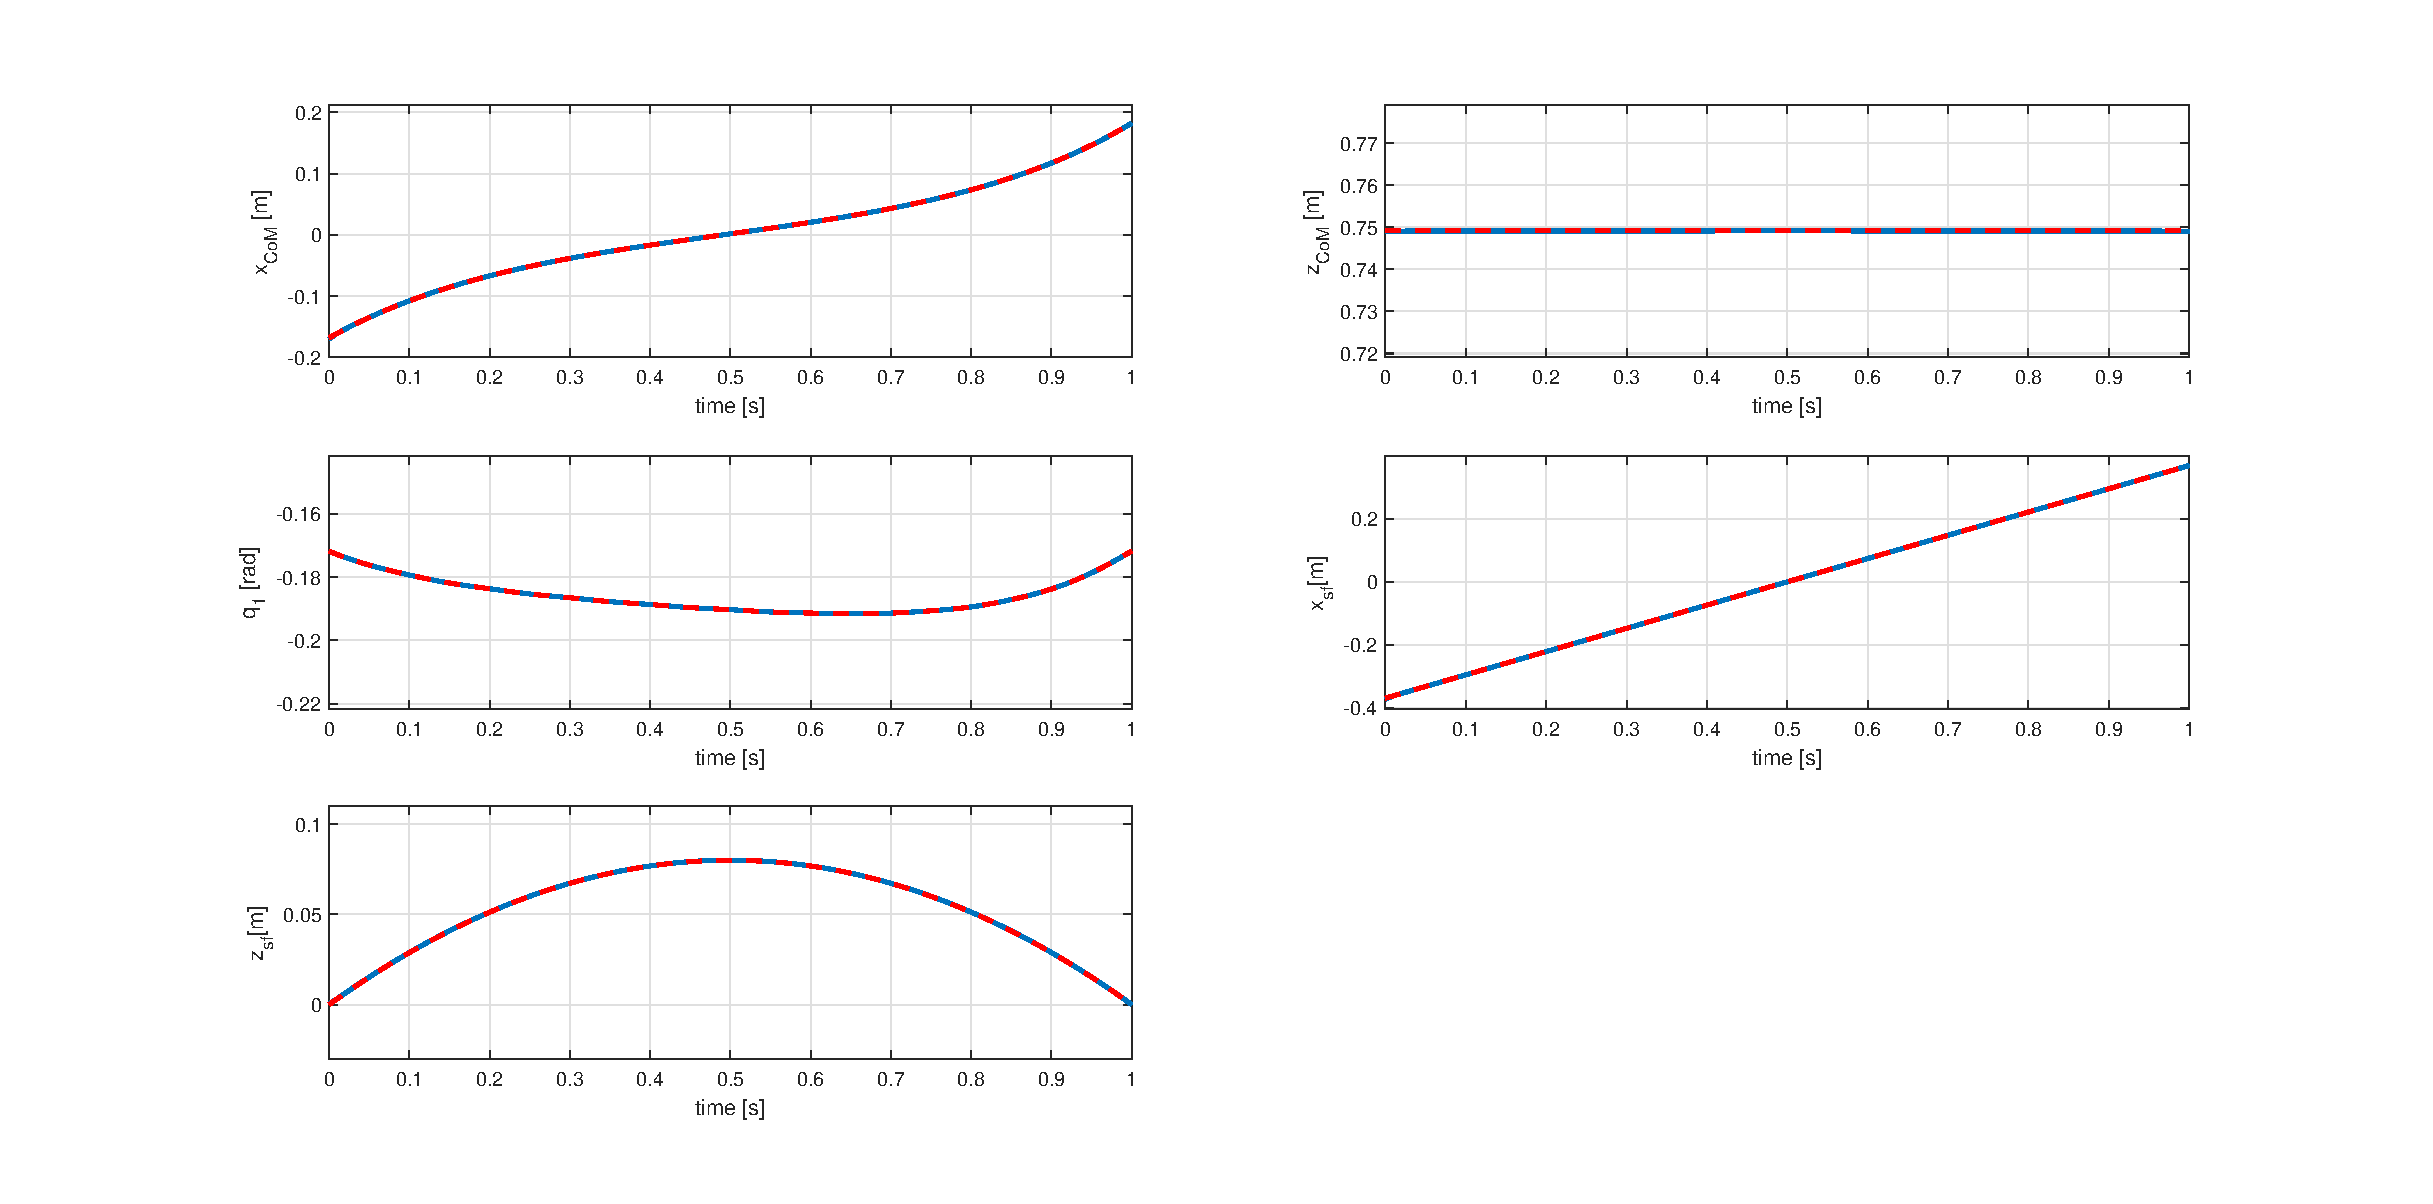
\includegraphics[width=1\linewidth]{Images/tracking_2_steps_1_sec.eps}
\label{fig:trajectory_tracking}
\caption{Tracking Result}
\end{figure}

\newpage
\section{Comparisons}

In this section a comparison between the results obtained through the two different methods is made.

The experiment setting is the same for both cases, so the duration of the step is 0.5 [s], while its amplitude is set to $0.37$ [m]. In order to compare the two techniques, RABBIT generalized coordinates values and their velocities during two complete steps are shown 

\begin{figure}[H]
\centering
\subfloat[Bounded CoM Tracking Coord.]{
\includegraphics[width=.4\linewidth]{Images/ste_pos.jpg}
\label{fig:ste_pos}
} \quad
\subfloat[Trajectory Optimization Coord.]{
\includegraphics[width=.4\linewidth]{Images/wrona_pos.jpg}
\label{fig:wrona_pos}
}
\caption{Comparison Generalized Coordinates}
\end{figure}

It is important to note that the CoM trajectories in both cases are very similar, even if at the end of the second step the CoM horizontal position of the FROST simulation is a little bit bigger. 

Another strong similarity can be seen in the profiles of the torso orientation. This is expected since in the second approach the task execution is always quite accurate and the reference was chosen as the same one of the FROST experiment.

On the other hand, the heights of the CoM are quite different in the two cases. In the first technique, this coordinate follows a parabola at each step, which is the result of the optimization criteria in order to follow the joint trajectory and it results in a more natural gait. On the other hand, in the second case its value is set to a fixed value, given the assumption made by the LIP model.
 
Regarding the legs coordinates, instead, it is worth noting that the profiles are quite different in the two cases, even if at the step instants the values are almost the same in the 2 approaches. Moreover, it is quite evident that the joint profiles are actually smoother when the trajectory optimization is employed and this can be seen especially on the joints $q_{31},q_{32},q_{41}$.

\begin{figure}[H]
\centering
\subfloat[][Bounded CoM Tracking Vel.]{
\includegraphics[width=.4\linewidth]{Images/ste_vel.jpg}
\label{fig:ste_vel}
} \quad
\subfloat[][Trajectory Optimization Vel.]{
\includegraphics[width=.4\linewidth]{Images/wrona_vel.jpg}
\label{fig:wrona_vel}
}
\caption{Comparison Generalized Coordinates Velocities}
\end{figure}

Regarding the velocities, also in this case the two outputs are quite different. It is important to notice that in both cases at the step instants one can find jumps in velocity, whereas the joints coordinates have continuous values and this was expected, given the impact model employed in this work.

Moreover, another important difference that stands out from these profiles is that in general the velocity magnitude is bigger in the second approach than in the trajectory optimization and this could be translated, by using the inverse dynamics approach, in an higher control effort required by the first technique.

\subsection{MATLAB animation}

In order to visualize in a more realistic way the joint trajectories, an animation--based simulation has been performed, using the FROST animator in MATLAB environment. Here five snapshots per each movie are shown. The main difference between the two groups of snapshots is the CoM trajectory (in green). The one derived from the feedback linearization and optimization approach is like a parabola, since the CoM height is not constant. On the other hand, the CoM trail in the animation coming from the kinematics tracking method is constant, as expected. 

\begin{figure}[H]
\centering
\subfloat[Step begins]{
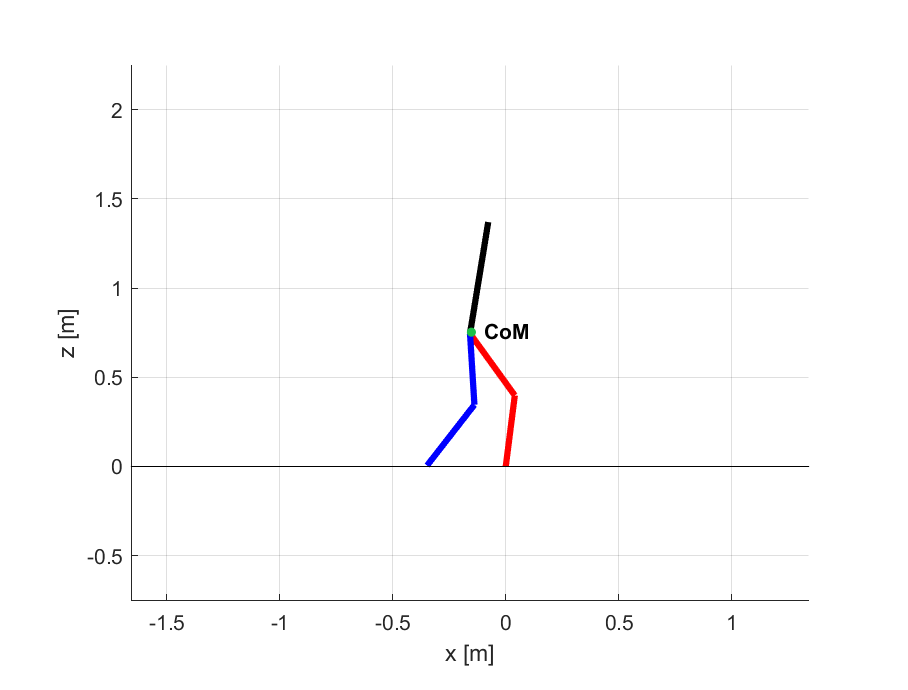
\includegraphics[width=.45\linewidth]{Images/Snapshots/FROST_1.eps}
} \quad
\subfloat[]{
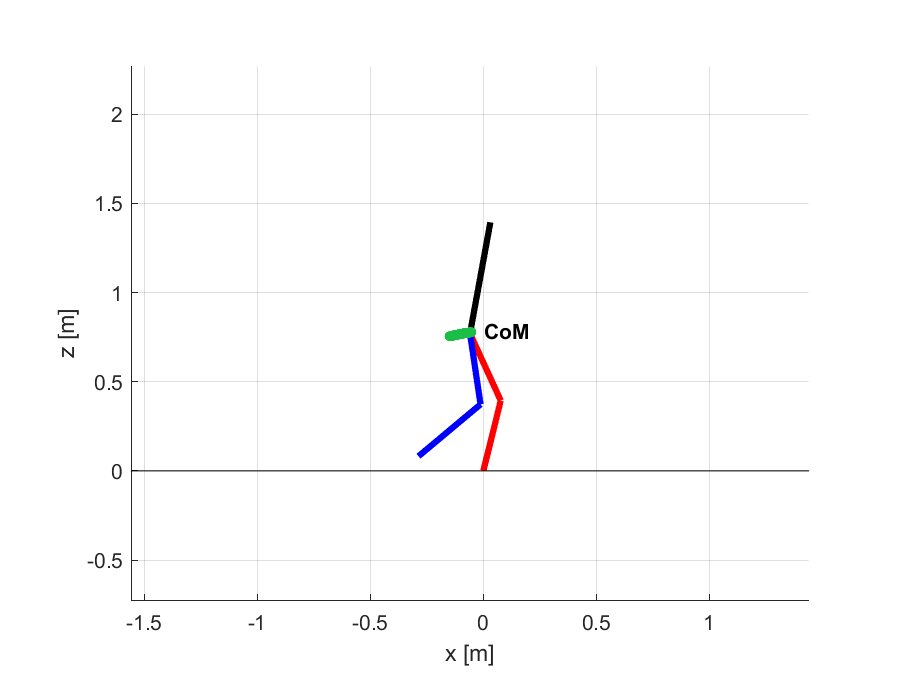
\includegraphics[width=.45\linewidth]{Images/Snapshots/FROST_2.eps}
} \\
\subfloat[][Maximum height of the swing foot]{
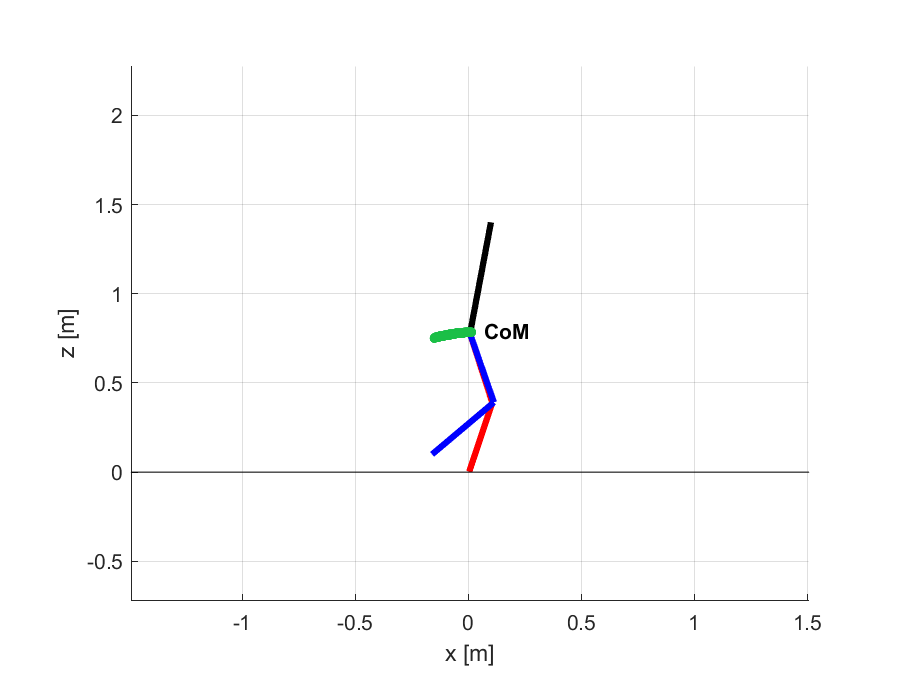
\includegraphics[width=.45\linewidth]{Images/Snapshots/FROST_3.eps}
} \quad
\subfloat[]{
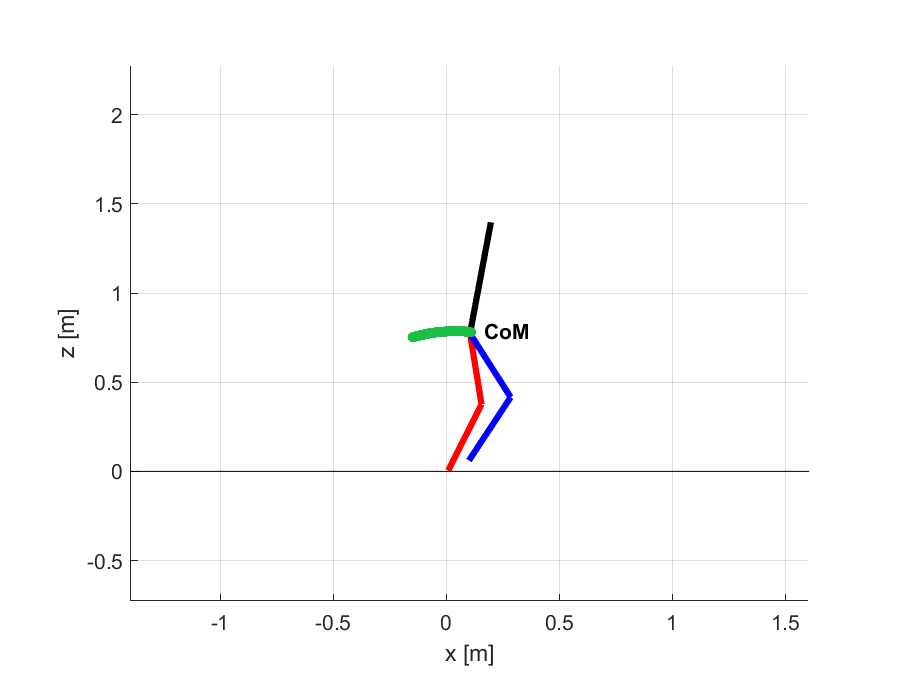
\includegraphics[width=.45\linewidth]{Images/Snapshots/FROST_4.eps}
} \\
\subfloat[Step ends]{
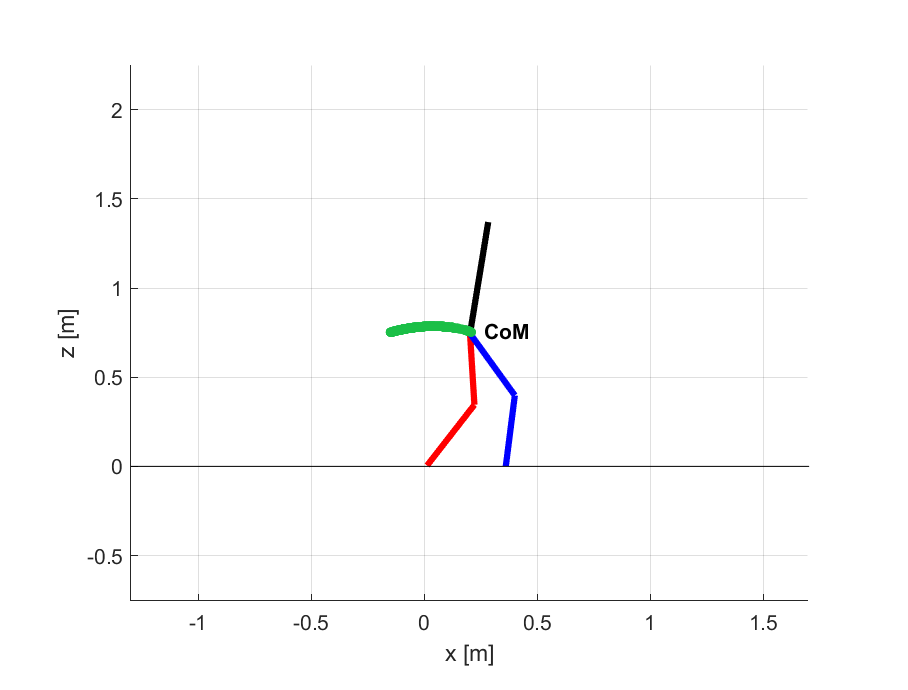
\includegraphics[width=.45\linewidth]{Images/Snapshots/FROST_5.eps}
}
\caption{Snapshots taken from hybrid trajectory optimization results. In green the CoM trajectory.}
\end{figure}


\begin{figure}[H]
\centering
\subfloat[Step begins]{
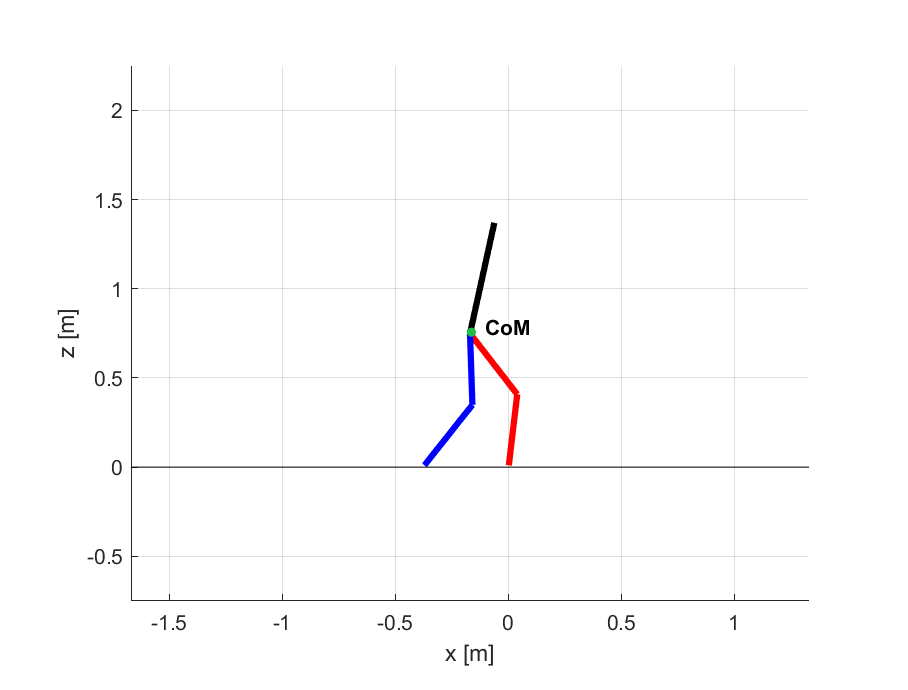
\includegraphics[width=.45\linewidth]{Images/Snapshots/Tracking_1.eps}
} \quad
\subfloat[]{
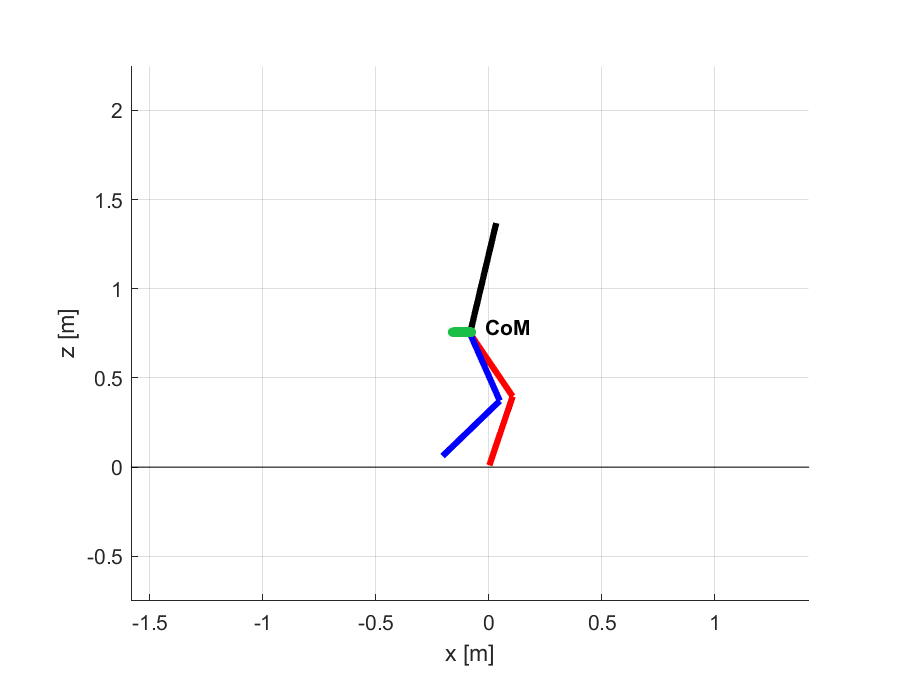
\includegraphics[width=.45\linewidth]{Images/Snapshots/Tracking_2.eps}
} \\
\subfloat[][Maximum height of the swing foot]{
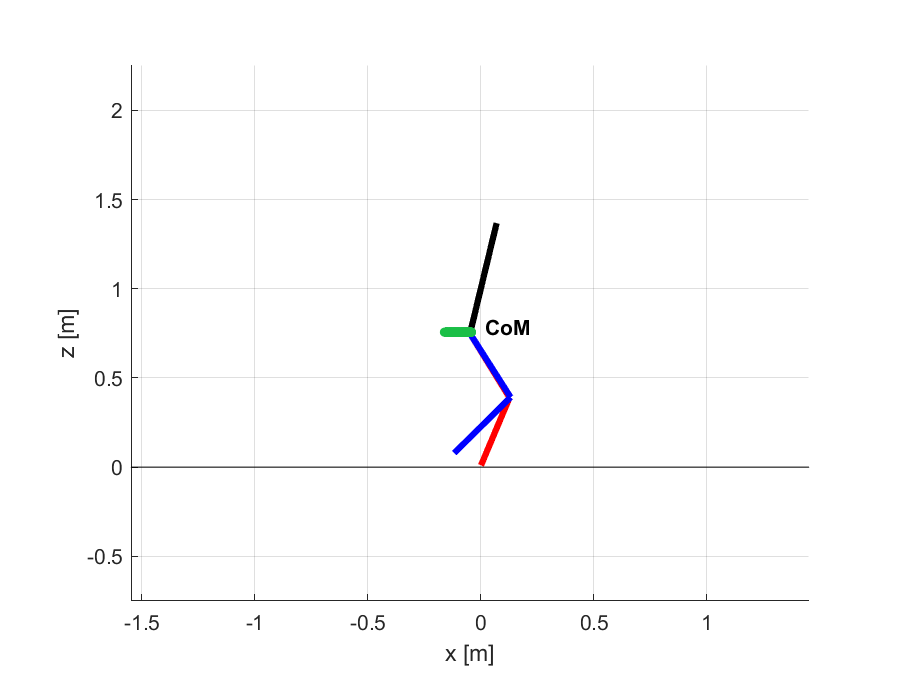
\includegraphics[width=.45\linewidth]{Images/Snapshots/Tracking_3.eps}
} \quad
\subfloat[]{
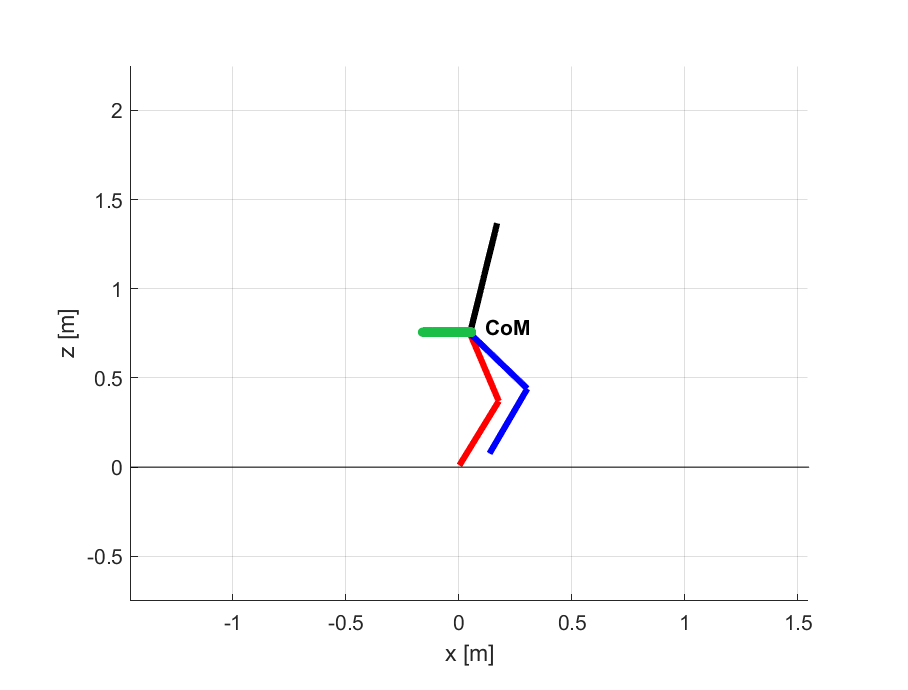
\includegraphics[width=.45\linewidth]{Images/Snapshots/Tracking_4.eps}
} \\
\subfloat[Step ends]{
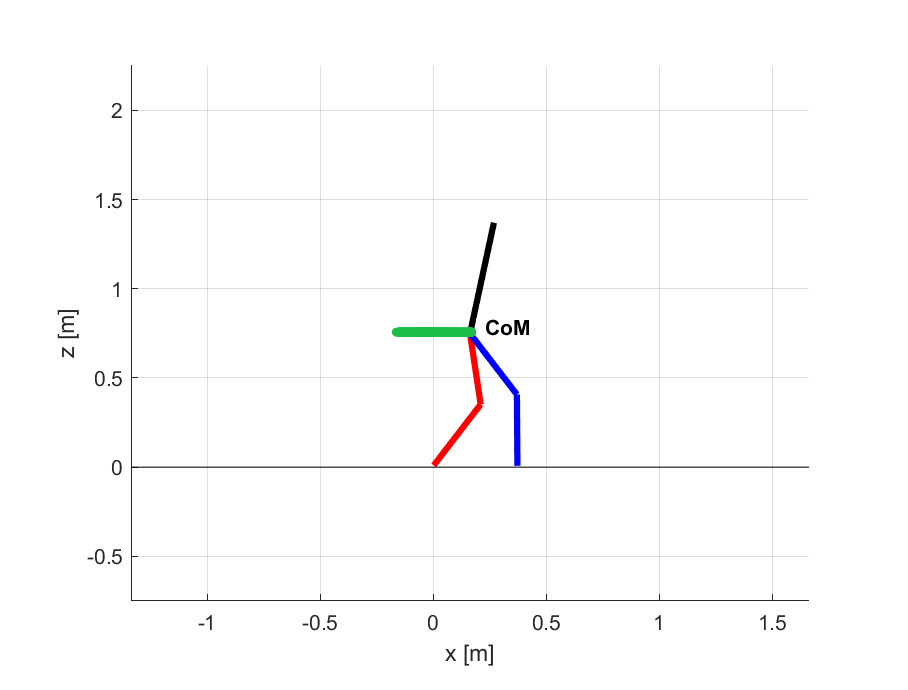
\includegraphics[width=.45\linewidth]{Images/Snapshots/Tracking_5.eps}
}
\caption{Snapshots taken from differential kinematics tracking results. In green the CoM trajectory.}
\end{figure}


\section*{Conclusions}

In this work, two different approaches to generate stable locomotion trajectories for planar biped walkers have been considered. The first one involves the dynamic model of the robot, and in particular relies on the feedback linearization technique. By using this method, one can design a parameterized output driving it to zero. Moreover, under some assumptions on the shape of $y=h(q)$, the input--output behaviour is decoupled, i.e. each external input acts only on one output. The optimization of the parameters used in the output functions, under some appropriate constraints which define the gait style, has been made using the MATLAB toolbox FROST and the NLP solver IPOPT. The results show a low control effort thanks to the minimization of the control energy. Moreover, the joint trajectories define a human-like gait.

The second approach relies only on the direct and differential kinematics of the robot. The LIP model has been used to generate CoM trajectories for the robot. This 2--dim task has been enriched by adding three more task: one for the torso orientation and two for the swing foot trajectory. Then, the jacobian of this stacked task has been built, and the joint velocities have been derived using the inverse differential kinematics relation. Thanks to this task augmentation the overall tracking error is negligible. By integrating these velocities, one gets the joint trajectories, which can be compared with those of FROST: the gait is very similar to the one derived with the optimization technique, but in this case the locomotion style is far from human-like walking, since the CoM height is kept constant. Hence, there will be more control effort at the femurs actuators because those links are the ones which need to define a larger trajectory in order to preserve the stability of the robot.

Eventually, it can be concluded that the optimization via parameterized feedback linearization is a more powerful method, since it provides directly the torque command for the DC motors, that is it does not rely just on velocities command. This property can be very useful when one needs to execute the locomotion on the real robot.

\newpage

\begin{thebibliography}{20}

\bibitem{rabbit}
Chevallereau C., Abba G., Aoustin Y., Plestan F., Westervelt E.R.,
Canudas-de-Wit C., Grizzle J.W., (2003), \textit{RABBIT: A Testbed for Advanced Control Theory. Designing, building, and controlling an experimental platform for the study of walking}, IEEE Control Systems Magazine, pp. 57-79.

\bibitem{frost}
Hereid A., Ames A. D., (2017), \textit{FROST: Fast robot optimization and simulation toolkit}, IEEE/RSJ International Conference on Intelligent Robots and Systems (IROS), Vancouver, BC, pp. 719-726.

\bibitem{isidori}
Isidori A., (1995), \textit{Nonlinear Control Systems}, Springer-Verlag, London. 

\bibitem{lanari2}
Lanari L., Hutchinson S., (2015), \textit{Planning Desired Center of Mass and Zero Moment Point Trajectories for Bipedal Locomotion}, IEEE-RAS 15th International Conference on Humanoid Robots (Humanoids), Seoul, pp. 637-642.

\bibitem{lanari}
Lanari L., Hutchinson S., Marchionni L., (2014), \textit{Boundedness issues in planning of locomotion trajectories for biped robots}, IEEE-RAS International Conference on Humanoid Robots, Madrid, pp. 951-958.

\bibitem{scianca}
Scianca N., Modugno V., Lanari L., Oriolo G., (2017), \textit{Gait generation via intrinsically stable MPC for a multi-mass humanoid model}, IEEE-RAS 17th International Conference on Humanoid Robotics (Humanoids), pp. 547-552.

\bibitem{westThesis}
Westervelt E. R., (2003), \textit{Toward a Coherent Framework for the Control of Planar Biped Locomotion}, PhD Thesis -- University of Michigan.

\bibitem{westBook}
Westervelt E. R., Grizzle J. W., Chevallereau C., Choi J. H., Morris B., (2017), \textit{Feedback control of dynamic bipedal robot locomotion}, CRC press, Boca Raton.

\bibitem{westervelt}
Westervelt E. R., Grizzle J. W., Koditschek D. E., (2003), \textit{Hybrid Zero Dynamics of Planar Biped Walkers}, IEEE Transactions on Automatic Control, Vol. 48, No. 1, pp. 42-56.

\end{thebibliography}

\end{document}